%  LaTeX support: latex@mdpi.com
%  In case you need support, please attach all files that are necessary for compiling as well as the log file, and specify the details of your LaTeX setup (which operating system and LaTeX version / tools you are using).

%=================================================================
\documentclass[energies,article,submit,moreauthors,pdftex]{Definitions/mdpi}
% \documentclass[preprints,article,accept,moreauthors,pdftex]{Definitions/mdpi}

%=================================================================
\firstpage{1}
\makeatletter
\setcounter{page}{\@firstpage}
\makeatother
\pubvolume{xx}
\issuenum{1}
\articlenumber{5}
\pubyear{2020}
\copyrightyear{2020}
%\externaleditor{Academic Editor: name}
\history{Received: date; Accepted: date; Published: date}
%\updates{yes} % If there is an update available, un-comment this line

%% MDPI internal command: uncomment if new journal that already uses continuous page numbers
%\continuouspages{yes}


%=================================================================
% Add packages and commands here. The following packages are loaded in our class file: fontenc, inputenc, calc, indentfirst, fancyhdr, graphicx,epstopdf, lastpage, ifthen, lineno, float, amsmath, setspace, enumitem, mathpazo, booktabs, titlesec, etoolbox, tabto, xcolor, soul, multirow, microtype, tikz, totcount, amsthm, hyphenat, natbib, hyperref, footmisc, url, geometry, newfloat, caption

\usepackage{subcaption}
\usepackage{tcolorbox}
\usepackage{tabularx}

%=================================================================
%% Please use the following mathematics environments: Theorem, Lemma, Corollary, Proposition, Characterization, Property, Problem, Example, ExamplesandDefinitions, Hypothesis, Remark, Definition, Notation, Assumption
%% For proofs, please use the proof environment (the amsthm package is loaded by the MDPI class).

%=================================================================
% Full title of the paper (Capitalized)
\Title{Design, Implementation, and Evaluation of Open Power Quality}

% Authors, for the paper (add full first names)
\Author{Anthony J. Christe, Sergey Negrashov and Philip M. Johnson}

% Authors, for metadata in PDF
\AuthorNames{Anthony J. Christe, Sergey Negrashov and Philip M. Johnson}

% Affiliations / Addresses (Add [1] after \address if there is only one affiliation.)
\address{%
Department of Information and Computer Sciences\\
University of Hawaii at Manoa\\
Honolulu, HI 96822\\
johnson@hawaii.edu}

% Abstract (single paragraph, 200 words max, background, methods, results, conclusions. Currently 193 words.)

\abstract{Modern electrical grids are transitioning from a centralized generation architecture to an architecture which must accomodate distributed, intermittent generation.  This transition also means that the formerly sharp distinction between energy producers (i.e. utility companies) and consumers (residences, businesses, etc) are blurring: residences can now both produce and consume energy, making energy policy more complex. The Open Power Quality (OPQ) project began in 2013 with the goal of designing and implementing a low cost, distributed power quality sensor network in order to provide make useful information about electrical grids available to producers, consumers, and policy makers.  Since then, we have designed low cost hardware devices that monitor power quality  and low-cost cloud-based software services that can economically analyze the data and detect a variety of anomalies. In 2019, we performed a pilot study where 15 OPQ hardware devices were deployed across the University of Hawaii microgrid for three months.  Results of the pilot study provide evidence that OPQ provides a variety of useful monitoring services and that the system could be scaled to service larger geographic regions. We conclude that OPQ provides a new and useful approach to power quality monitoring.}

% Keywords
\keyword{Power Quality, Open Source, Renewable Energy, Grid Stability}


\begin{document}

\section{Introduction}

%{\em The introduction should briefly place the study in a broad context and highlight why it is important. It should define the purpose of the work and its significance. The current state of the research field should be reviewed carefully and key publications cited. Please highlight controversial and diverging hypotheses when necessary. Finally, briefly mention the main aim of the work and highlight the principal conclusions.}

\subsection{Motivation}

Power quality is not currently a concern for most people in developed nations. Just like most people in developed nations assume that their tap water is of adequate quality to drink, most also assume that their electricity is of adequate quality to power their homes and appliances without causing harm. And, in both cases, most people assume that public utilities will appropriately monitor and correct any quality problems if they occur.

Successfully maintaining adequate power quality and providing sufficient amounts of it to meet the rising needs of consumers has been a triumph of electrical utilities for over 100 years. In recent times, however, there have been changes to the nature of electrical generation and consumption that make power quality of increasing concern and interest. First, there is a global need to shift to renewable energy sources. Second, traditional top-down grid power quality monitoring may not be well suited to bottom-up, distributed generation associated with renewable energy sources such as roof-top solar. Third, modern consumer electronics place more stringent demands on power quality.  Finally, effective public policy making in this modern context can be aided by public access to power quality data.  Let's look at each of these in a bit more detail.

{\em 1. We need more renewable energy.} Concerns including pollution, environmental degradation, and climate change have produced a global movement away from centralized, fossil-fuel based forms of electrical energy generation and toward distributed, renewable alternatives such as wind and solar. But the economic, environmental, and political advantages of renewable energy comes with significant new technical challenges. Wind and solar are intermittent (for example, solar energy cannot be harvested at night) and unpredictable (for example, wind and solar energy fluctuate based upon cloud cover and wind speed). In addition, renewable energy generation is often distributed throughout the grid (such as in the case of residential rooftop photovoltaic (PV) systems).

One impact of adding renewable energy generation to an electrical grid is that maintaining adequate power quality is much more challenging. This problem is inversely proportional to the size of the electrical grid. For example, each island in the State of Hawaii maintains its own electrical grid, ranging from a 1.8 GW grid for the island of Oahu to a 6 MW grid for the island of Molokai.  (In contrast, the size of the European electrical grid is approximately 600 GW and the size of the U.S. continental grid is over 1000 GW.) For small grids, the unpredictable nature of power generation by distributed, intermittent renewables can quickly create problems for grid stability. In the case of Hawaii, consumer demand for grid-tied rooftop solar exceeded the ability of Hawaiian Electric to manage, resulting first in complex and expensive "interconnection studies" \cite{trabish_solar_2014,anastasi_energy_2009}, and later in the requirement for new installations to include batteries and grid-disconnected operation.

{\em 2. Traditional top-down monitoring is not well-suited to bottom-up energy generation.} For traditional grid architectures where generation is centralized and under the complete control of the utility, it is common to monitor power quality only to the substation level, because it can be assumed that the power quality experienced at the substation is a reasonably accurate proxy for the power quality experienced by the 1,000 or so end-users serviced by the substation. Furthermore, if an end-user experiences a power quality problem not experienced by the substation, then it is mostly likely due to equipment or electrical issues local to that end-user and not a grid-level problem.

These assumptions might not hold in grids with distributed, intermittent generation by end-users, such as is the case with roof top solar. In these cases, the unpredictable nature of generation can lead to local power quality problems that are not experienced by the substation, and that are not due to any single individual, but rather the bottom-up power generation architecture of the grid. Nakafuji notes that Hawaiian Electric is contending with PV penetrations in excess of 60\% on certain distribution circuits, for which traditional rules of thumb for design of protection and distribution systems might not hold \cite{nakafuji_back--basics_2011}.

{\em 3. Consumer electronics require higher quality power.} The rise of consumer electronics has raised the bar for what constitutes ``adequate" power quality. Only a few decades ago, computers were a rare presence outside of labs and large institutions. Today, computers are everywhere: embedded in phones, washers, refrigerators, thermostats, and so forth. These electronic devices not only have higher power quality requirements, but some of them actually introduce power quality problems in the form of harmonic distortion. Poor power quality can result in electronic devices failing unpredictably, and/or decreasing their lifespan.

{\em 4. Power quality data should be publicly available.} Electrical utilities are not required to be totally transparent about the quality of power they provide to consumers. For example, in Hawaii, utilities are required to make a "best effort" to provide non-harmful voltage and frequency values, but are only required to publicly report on power outages of more than 3 minutes. There is no requirement for utilities to report potentially harmful levels of voltage, frequency, THD, or transients as long as they do not lead to outages. Indeed, in places like Hawaii, there is not yet infrastructure in place to enable utilities to collect that information, even if they were asked to report on it.

Providing power quality data to address the above issues requires solving several difficult technical problems. First, monitoring below the substation level increases the number of required monitoring devices by two to three orders of magnitude. This has significant implications for the cost of monitoring in terms of the devices, and the sheer amount of low-level power quality data that will be produced. Second, this low-level data must be processed in a manner that does not require inordinate amounts of processing, network bandwidth, or storage. Finally, collecting the data is not useful if it cannot be converted into actionable information in a reasonable amount of time.

\subsection{Goals of the Open Power Quality Project}

The goal of the OPQ Project is to provide a scalable source of actionable power quality data about electrical grids, particularly those with high levels of distributed, intermittent power generation. OPQ accomplishes this through the design and implementation of a low-cost sensor network for power quality using custom power quality monitors with real-time, two way communication to a set of cloud-based services. An OPQ sensor network is designed to be useful to consumers who want to better understand the performance of their public utilities, to researchers who wish to design improvements to grid management, and to public policy makers responsible for designing and implementing regulatory frameworks for electrical utilities.  There are several key features of our project emerge from these goals.

{\em OPQ Box.} First, our custom power quality monitoring hardware device, called "OPQ Box" can be produced for approximately US\$75. This is from 10 to 100 times less expensive than commercial power quality monitors. This cost differential means, for example, that instead of monitoring power quality at the level of individual buildings, OPQ makes it economically feasible to monitor power quality on each floor or even in each room of a building. Similarly, instead of monitoring power quality at the substation level of the grid, OPQ Boxes make it feasible to deploy dozens or hundreds into a community to obtain fine-grained data about the impact of solar or other renewables as directly perceived by the customer.

{\em Cloud-native information architecture.} Second, our information architecture is "cloud native", which means that OPQ Boxes are not designed for stand-alone, autonomous use, unlike current commercially available power quality monitors. Instead, our hardware boxes and cloud-based services perform real-time, two-way communication over the Internet to determine what power quality data must be gathered and with what fidelity in order to most efficiently produce actionable information. Two-way communication between the OPQ Boxes and could services creates the ability to control individual OPQ Boxes based upon the global state of all OPQ Boxes in an OPQ sensor network. As a result, OPQ cloud services can obtain and analyze high fidelity wave form data only when desired, without the prohibitive network overhead of constantly communicating this data from boxes to the cloud. This enables OPQ installations to be simultaneously responsive and scalable.

{\em Plug-in analysis architecture.} Third, all OPQ software services are designed for extensibility and interoperation. Our middleware components (Mauka and Makai) provide a plugin architecture. Our visualization component (View) is built from modular UI elements using React.  This means that OPQ is not a monolithic, closed system with a frozen feature set, but rather a design environment for experimentation with advanced classification and analysis of power quality data.

{\em Open Source.} Fourth, our software and hardware designs and implementations are made available using open source licenses. This means that organizations choosing OPQ do not face the business risk of committing resources to a single vendor with proprietary hardware and software. Our goal is to facilitate the creation of a community of researchers and industry practitioners to replicate, extend, and apply the insights gained from the OPQ system.

While we believe OPQ offers a compelling combination of capabilities, we want to be clear that all network designs involve trade-offs. As we will show below, other commercial and research solutions have features not provided by OPQ that may be important depending upon an organization's specific needs. In some cases, OPQ may not be the appropriate choice. In other cases, a hybrid solution consisting of OPQ in combination with other technologies for power monitoring may be most appropriate.

\subsection{Structure of this paper}

The next sections present an overview of the OPQ system architecture and information architecture. The following section presents related research and technology.  Section \ref{sec:makai} provides more detail on the OPQ Box, and Section \ref{sec:makai} provides more detail on our cloud services. Section \ref{sec:pilot} discusses the pilot deployment of a sensor network and its results. We conclude in Section \ref{sec:conclusion} with some proposals for future research.



\section{Methods}

The central aim of the OPQ Project is to provide a scalable source of actionable power quality data about electrical grids, particularly those with high levels of distributed, intermittent power generation.

Our research methodology consists of three (potentially interleaved) phases. First, we specify, design, and implement novel hardware and software for collecting, transmitting, and analyzing four essential measures of power quality data: voltage, frequency, THD, and transients. Second, we verify that our implementation matches our specifications through laboratory experiments.  Third, we validate our implementation by testing a variety of hypotheses through a real-world deployment. In this paper, we report on results from a pilot deployment at the University of Hawaii over the course of three months.

Our central hypothesis is that we can accomplish this through the design and implementation of a low-cost sensor network for power quality using custom power quality monitors with real-time, two-way communication to a set of cloud-based services.

We will test this central hypothesis through six subhypotheses: (1) OPQ provides valid and reliable collection of power quality data (Section \ref{hyp:01}), (2) OPQ's triggering system provides advantages with respect to bandwidth and computation (Section \ref{hyp:02}, (3) OPQ enables subthreshold event detection based upon temporal locality (Section \ref{sec:subthreshold-events}), (4) The OPQ information architecture provides a means to produce actionable insights (Section \ref{hyp:04}), (5) the OPQ information architecture provides predictable upper bounds on storage resources (Section \ref{hyp:05}), and (6) OPQ provides useful adaptive optimization capabilites (Section \ref{sec:adaptive-optimization}).

The remainder of this section presents the overall architecture of OPQ, along with details on the design and implementation of each of the principal architectural components. We will also discuss our verification activities for each component. Our validation and hypothesis testing activities will be described in Section \ref{sec:pilot-study}.

\subsection{OPQ Architecture}

The OPQ system architecture consists of four major open source hardware and software components that provide end-to-end support for the capture, triggering, analysis, and reporting of consumer level local and global PQ events.  OPQ Box is a hardware device that detects the electrical waveform from a standard residential outlet and communicates both low and high fidelity representations of the waveform to other OPQ system components either at predefined intervals or upon request. OPQ Makai monitors incoming low fidelity data from OPQ Boxes, requests high fidelity data when necessary, and stores the results in a MongoDB database. OPQ Mauka analyzes low level data and analyzes it to produce higher-level representations according to the information architecture described below, and can tell OPQ Makai to request high fidelity data from one or more OPQ Boxes to facilitate analysis. OPQ View is a browser-based visualization platform for displaying the results for data capture and analysis.

\begin{figure}
\center 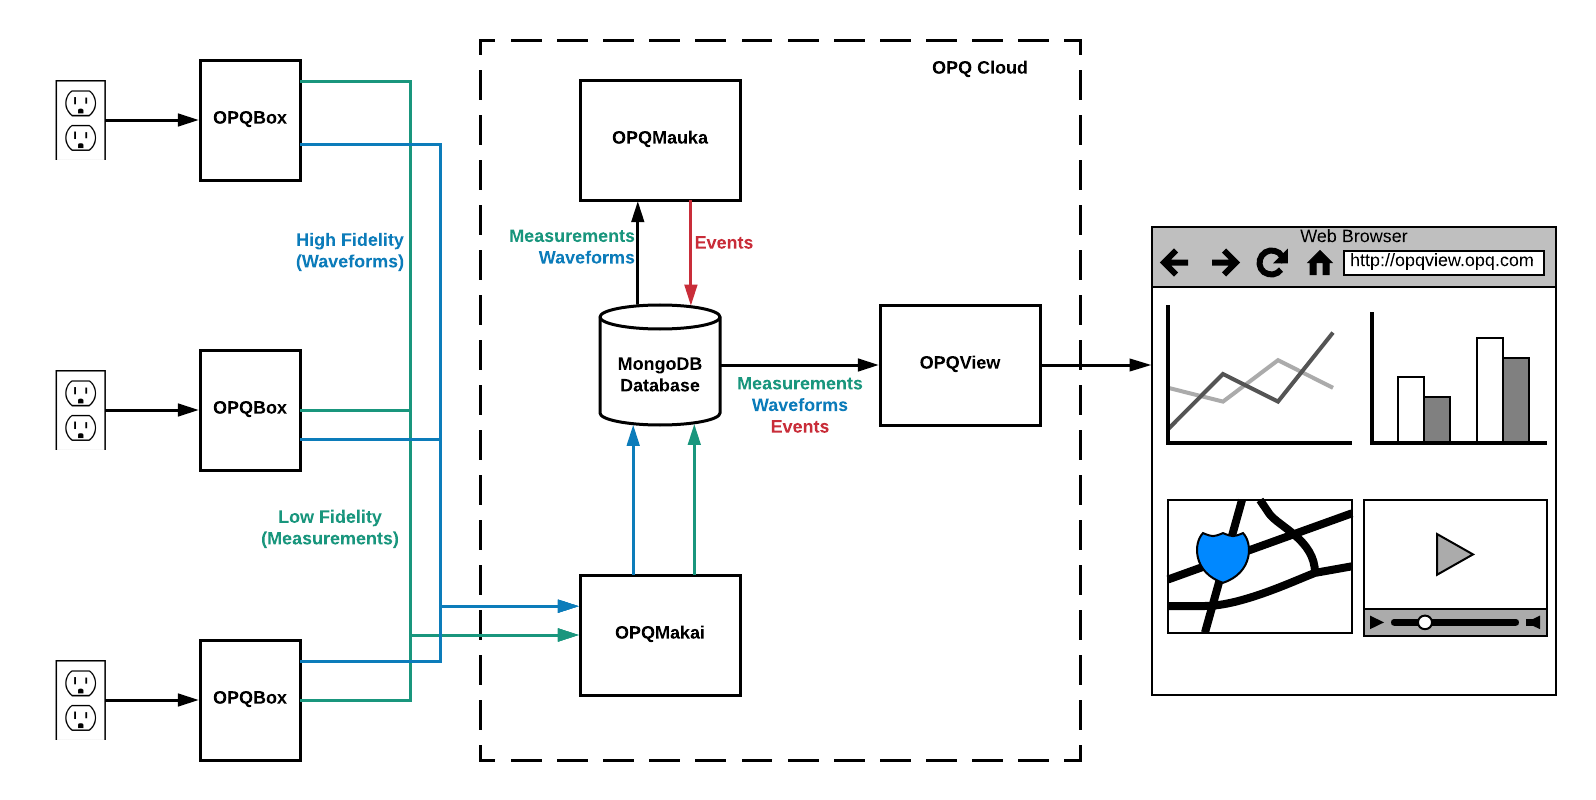
\includegraphics[width=5in]{images/architecture/system-diagram.png}
\caption{High level system architecture of an OPQ Sensor Network}
\label{fig:architecture}
\end{figure}

Figure \ref{fig:architecture} illustrates how these components work together to take information from wall outlets (on the left side) to the display of analyses in a browser (on the right hand side).  First, OPQ Boxes analyze power from wall outlets, and send low fidelity measurements to OPQ Makai. OPQ Makai analyzes low fidelity measurements, and requests high fidelity waveforms when desirable. Both measurements and waveforms are saved in a MongoDB database. OPQ Mauka analyzes low and high fidelity data, and creates "events" to represent anomalies. OPQ View notifies users of events and allows them to drill down into low and high fidelity data.

OPQ Makai, OPQ Mauka, and OPQ View are all cloud-based software services that collectively form a single "instance" with respect to data transmission, storage, analysis, and visualization. We refer to this collection of software-side components as OPQ Cloud. Every OPQ Box connects to a single instance of an OPQ Cloud. It is possible to have multiple OPQ Cloud instances. For example, a company might install an OPQ Cloud instance behind their firewall along with OPQ Boxes to provide a private mechanism for collecting and analyzing power quality data.

\subsection{OPQ Box}
\label{sec:opq-box}

OPQ Box is a hardware device designed to provide inexpensive, extensible and accurate residential power quality measurements.
A block diagram of OPQ Box is shown in Figure~\ref{fig:opq:1:1}.
A complete device is shown in Figure~\ref{fig:opq:1:2}.

\begin{figure}[ht]
	\centering
	\begin{subfigure}{.5\textwidth}
	  \centering
	  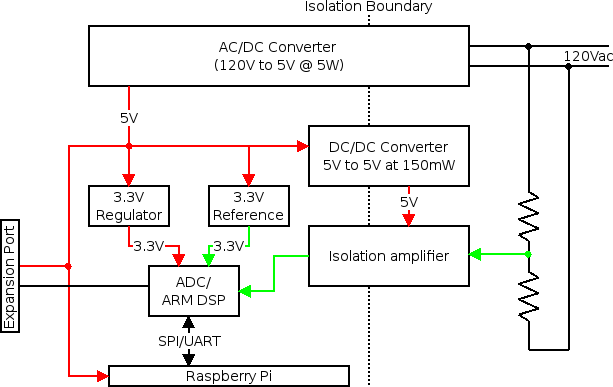
\includegraphics[width=0.9\linewidth]{images/opq-box/opqbox_diagram.png}
	  \caption{OPQ Box Block Diagram.
	  The power path is in red, signal path is in green and the digital IO is in black.}
	  \label{fig:opq:1:1}
	\end{subfigure}%
	\begin{subfigure}{.5\textwidth}
	  \centering
	  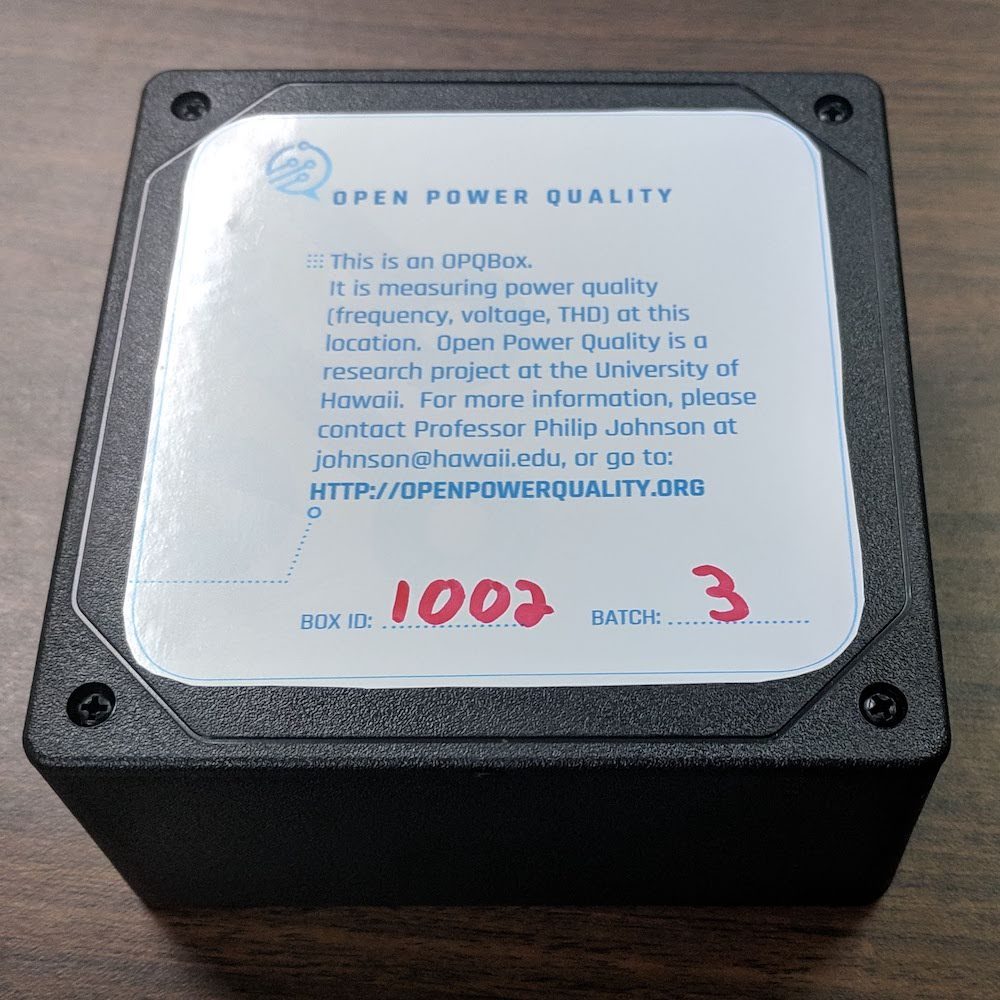
\includegraphics[width=0.7\linewidth]{images/opq-box/opqbox_photo.jpg}
	  \caption{OPQ Box in an ABS plastic enclosure.}
	  \label{fig:opq:1:2}
	\end{subfigure}
	\caption{(a) OPQ Box block diagram and (b) production OPQ Box ready for deployment}
	\label{fig:opq:2}
\end{figure}

\subsubsection{OPQ Box Hardware}\label{subsec:hardware}

The power system of the OPQ Box electrically isolates most of the device from the AC mains power.
An isolated AC-DC converter generates $5V_{dc}$ from the mains $120V_{ac}$.
5V is used to power the Raspberry Pi, the equipment connected to the expansion port, the 3.3V regulators and voltage reference, and an isolated DC/DC converter.
3.3V is used to power the isolated end of the isolation amplifier as well as the STM32F3 analog to digital converter/digital signal processor (ADC/DSP).
The hot side of the isolation amplifier is powered from the isolated DC/DC converter.
This allows OPQ Box to function with a battery attached to the expansion port, so that it may retain data and continue to operate during a power outage.

\begin{figure}[ht]
  \begin{center}
  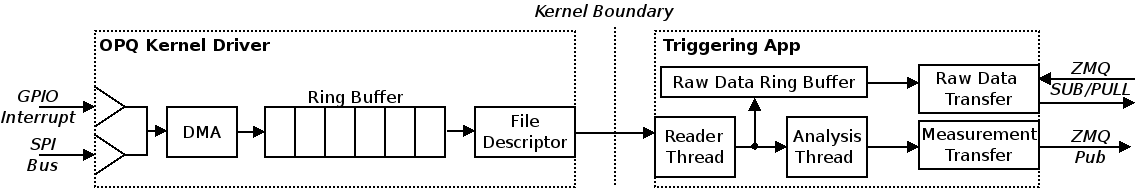
\includegraphics[width=0.9\textwidth]{images/opq-box/opqbox_software.png}
  \end{center}
  \caption{Block diagram of the OPQ Box 2 software stack.}
  \label{fig:opq:3}
\end{figure}

A Raspberry Pi single board computer (SBC) is responsible for signal analysis and anomaly detection.
The Raspberry Pi model used in OPQ Box is the Pi Zero W equipped with 256MB of main memory and a single core 1GHz ARM11 CPU. It also contains an on-board 802.11n WIFI transceiver, which removes the need for an external WIFI dongle.

\subsubsection{OPQ Box Software}\label{subsec:software}

The software stack of the Raspberry Pi aims to deliver an accurate and precise power quality analysis framework despite the rather limited capabilities of the hardware.
A block diagram of the software stack is shown in Figure~\ref{fig:opq:3}.
Digital data is transferred from the DSP to the Raspberry Pi via Serial Peripheral Interface, with the Pi acting as the master and the DSP as a slave device.
A hardware interrupt line is used to inform Pi software that the DSP is ready for the data transfer, and a kernel driver provides management of the SPI bus.
Internally, the OPQ driver maintains a ring buffer of 16 windows, each of which is 200 data samples in size.
Upon receiving the interrupt for the DSP, the CPU sets up the DMA transfer and the DMA engine transfers a 200 sample window into the kernel memory without CPU interaction.
This scheme requires the CPU to only service 60 interrupts a second, with each interrupt requiring on the order of 100 instructions, for a CPU utilization of less than $1\%$ in normal operation.
Userland applications communicate with the kernel driver using a file descriptor, where every $read$ system call yields 200 samples of raw waveform.
As a result, the smallest window that a userland application may process is a single AC cycle of the grid mains.

The userland component of the OPQ Box software is a multi-threaded extensible analysis framework called Triggering.
The reader thread is responsible for transferring and accumulating data from the kernel driver.
The smallest data buffer that the Triggering application processes at any given time is 10 grid cycles or 2k samples.
Once the cycles are transferred to the userland and timestamped, they are passed to the analysis thread for feature extraction, as well as to the Raw Data Ring Buffer (RDRB).
Since internally all data is addressed using shared pointers, during data duplication no copying is required.
RDRS is capable of buffering up to an hour of data before it is overwritten, resulting in the RDBS maximum size of 100MB.

The analysis thread of the Triggering application performs feature extraction of the raw data windows of 2000 samples.
Four metrics are extracted from the data stream: (1) Fundamental frequency, (2) RMS Voltage, (3) Total Harmonic Distortion, and (4) Transients. Let's briefly discuss how each of these are computed.

\subsubsection{OPQ Box: Calculating Fundamental Frequency}\label{subsec:fundamental-frequency}

The fundamental frequency is calculated by computing the zero crossings of the AC waveform.
In order to improve the accuracy of the frequency calculation one must first filter out as much noise as possible.
Since our sampling rate is quite high (12kSps) and the fundamental frequency is quite low (60Hz), it is very computationally expensive to perform this filtering in a single step.
Instead, filtering is accomplished via a set of two low pass finite impulse response (FIR) filters.
First filter has a passband of 0-600Hz allowing us to downsample the waveform to 1200 samples per second.
Next filter has a passband of 0-100Hz allowing for further removal of high frequency noise.
Finally, zero crossings are extracted and used for the frequency calculation.
The zero crossings themselves were calculated by using linear interpolation between two points which bracket the time axis.

\subsubsection{OPQ Box: Calculating RMS Voltage}\label{subsec:root-mean-square-voltage}

Root mean square voltage ($V_{rms}$) in electrical power is the equivalent value of DC voltage which would dissipate the same power in the resistive load. $V_{rms}$ is a convenient measure for detecting voltage sags and swells, since they result in nominally higher and lower computed value.

Similarly to the frequency calculation, OPQ Box uses a 10 cycle window for a single $V_{rms}$ calculation. Unlike the frequency calculation, the input is not filtered a priori.

\subsubsection{OPQ Box: Calculating THD}\label{subsec:thd}

The OPQ Box calculates total harmonic distortion (THD) using the industry standard methodology.
It should be noted that in the power quality domain THD is expressed as a percentage as opposed to $\frac{dB}{\sqrt{Hz}}$ as used in other disciplines.
Operationally, OPQ Box computes THD for 10 cycles of the fundamental frequency.
First an FFT transforms the real voltage samples into its frequency components.
Next, the square of the harmonic bins are accumulated and scaled by the magnitude of the fundamental power.

\subsubsection{OPQ Box: Transient Detection}\label{subsec:transient-detection}

OPQ Box transient detection is performed via filtering out of the fundamental frequency via an FIR high pass pass filter with a cutoff frequency of $400Hz$ and searching for a maximum value in the remainder.

It should be noted that this transient detection method is susceptible to THD fluctuations, since any harmonic above $400Hz$ will remain in the filtered waveform.
However, since the THD information is transmitted along with the transient detection metric, they can be correlated in downstream transient detection.

\subsubsection{OPQ Box: Network Communication}\label{subsec:network-communication}

The computed fundamental frequency and $V_{rms}$ are transmitted to the Makai service for aggregation.
Data transmission is handled using ZeroMq software stack with Curve25519 elliptic curve encryption.
Each device holds a unique private and public key, as well as the servers' public key, allowing both the Makai service and the OPQ Box to verify its peer.
Internally, metrics transmission uses ZeroMq's PUB/SUB protocol.
This protocol is a publish subscribe topology, with each message containing the topic and a payload.
Additionally, ZeroMq allows for multiple sub peers with subscriptions forwarded to the publisher automatically via a side channel.
This allows for the aggregation service to be spread across multiple nodes, with minimal network overhead.

If the aggregation service determines that an anomaly has occurred, it is able to request raw waveform from the OPQ Box RDRB via a separate ZeroMq pub sub channel.
If the RDRB buffer contains data for the requested temporal range, OPQ Box transmits the available data to the aggregation service via a push pull ZeroMq channel.
Protobuf message serialization is used to encode messages across the OPQ ecosystem.

In order to make a distributed measurement, all of the OPQ Boxes on the OPQ network need to maintain an accurate time reference.
Time synchronization across multiple OPQ Boxes is accomplished using the Network Time Protocol.
The expansion port of the OPQ Box supports a GPS receiver.
However, since GPS receivers require line of sight to the sky, it was not used for deployment.
NTP performance has been verified against GPS resulting in time error of $8ms\pm 5ms$ which is typical for NTP running over the Internet with a nearby NTP server.

\subsubsection{OPQ Box: Manufacturing}

Currently, there is no mechanism for mass production of OPQ Boxes, but all of the plans are available under an Open Source license, so interested organizations with some basic hardware engineering skills can build their own boxes.

Complete specifications for the OPQ Box hardware, firmware, and software are available \cite{negrashov_opq_2020}. As of the time of writing, a single OPQ Box can be manufactured for approximately \$100 in parts. The cost drops significantly with scale, for example, 100 OPQ Boxes can be manufactured for a cost of approximately \$75 in parts per device.



\subsection{OPQ Makai}
\label{sec:opq-makai}

OPQ Box provides an inexpensive hardware device for collecting four important power quality measures with high fidelity, but realizing its potential requires an innovative approach involving two-way communication between OPQ Boxes and the OPQ cloud-based services. To see why, consider the IEEE 1159 standard for single location power quality monitoring \cite{unruh_ieee_2018}.  For transient monitoring, IEEE 1159 suggests a sampling rate of at least 7680 samples/second, up to 1 Megasample/second. This implies that if the cloud service requires the high fidelity data from all OPQ Boxes, it would incur a very large bandwidth cost. At 20 Ksamples/second with 16bit samples, a single OPQ Box will generate 300Kb/second of network bandwidth. Several thousand devices would easily saturate a 1 GB network link. In addition, collecting and recording all of the raw waveform data from residential power quality meters could lead to security and privacy issues.

Network bandwidth saturation is a common problem for distributed sensor networks, and a common solution is called "self-triggering".  In this approach, each monitoring device is configured with a threshold value for one or more measures of interest. When the threshold for a measure of interest is exceeded, then and only then is data sent over the network to cloud-based services for analysis.

The problem with the self-triggering approach is that grid-wide power quality events do not affect the entire grid in the same way. For example, due to the grid’s hierarchical structure, a voltage sag on one sub-circuit can manifest as a sag of a different magnitude or even a swell on another \cite{kahle_power_2015}. This may result in a situation where some of the monitoring devices will not consider a power quality anomaly as an event, because it did not surpass the metric threshold, and simply ignore it. From an analysis perspective, however, it can be useful to get raw data from all of the affected devices, not just the ones that were the affected to the point where the box was triggered. This additional information can be used to localize the disturbance, as well as better evaluate its impact.

Since sending all the data is infeasible, and since the self-triggering approach can potentially miss important forms of information, OPQ implements a novel, hybrid centralized/decentralized data acquisition scheme which involves two-way communication between the OPQ Boxes and a cloud service called OPQ Makai. In this scheme, OPQ Boxes use local processing resources to feature extract the incoming waveforms while storing them locally for an hour. Each OPQ Box sends its feature data to OPQ Makai once a second, which we called the "triggering stream". Feature data is very small, on the order of a few kilobytes, and so this approach allows the sensor network to scale to thousands of devices with acceptable network bandwidth requirements.  OPQ Makai processes the incoming triggering stream and looks for anomalies. If an anomaly is present in only a single device, it is highly probable that the cause is local and not grid-level. On the other hand, if the triggering stream shows an anomaly temporally collocated across multiple devices, the entire network or a subset of the network may be queried for raw waveform data for a temporal region which corresponds to the disturbance in the triggering stream.

Our pilot study, discussed in Section \ref{sec:pilot-study} will provide examples of the novel analysis capabilities made possible by OPQ Box and OPQ Makai communication. In general, here are the main advantages of our hybrid centralized/decentralized approach over traditional self-triggering and the ``naive" approach of sending all of the data:

{\em Bandwidth usage is minimized.} Instead of sending the entirety of raw data, only extracted features are sent. This results in a tiny fraction of the bandwidth requirement when compared to raw waveforms. Furthermore, the temporal window which encompasses a single feature can be adjusted in real time. Thus, as soon as an anomalous behavior is observed in a subset of sensors, this window can be adjusted for a finer grained feature extraction.

{\em Effects of latency are minimized.} In this case, "latency" refers to the time required for OPQ Makai to process the incoming feature stream and decide whether to request high fidelity data from one or more OPQ Boxes. Even at 1M samples/second at 16 bits of resolution, the memory requirement to store 5 minutes of raw waveform without compression are on the order of 512MB, which is well within the realm of inexpensive single board computers such as Raspberry PI. With compression specifically suited to the signal of interest, the memory requirement can be reduced even further. In the case of the OPQ sensor network, OPQ Makai has an hour to process feature data and request high fidelity data from OPQ Boxes. During our pilot study, OPQ Makai always responded within a second or two.

{\em Cloud processing requirements are reduced.} Since feature extraction is already performed at the device level, cloud computation requirements are reduced. With the advent of the Internet of Things, the computational capacity of edge devices is increasing.

{\em Subthreshold data acquisition can improve understanding of grid-local anomalies.} OPQ Makai makes the decision to acquire raw waveform from OPQ Boxes. This allows analysis of data from devices which were only mildly affected or even not affected at all by the disturbance. This creates new possibilities for investigation of disturbance propagation across the sensed area, as will be discussed in Section \ref{sec:pilot-study}.

{\em Temporal locality allows OPQ to provide improved insights into power quality anomalies over traditional triggering algorithms.} By exploiting the idea of temporal locality, it is possible to ascertain the geographical extent of an anomaly with only coarse features. This allows for a simple robust algorithm which may be deployed at the sink node for anomaly detection.

\subsubsection{OPQ Makai: Design}

OPQ Makai is a distributed extensible microservice framework responsible for receiving the triggering stream from the OPQ Boxes, locating anomalous temporal regions and requesting raw waveform for the anomalous time ranges. As shown in Figure \ref{fig:makai-design}, Makai consists of four major components: Acquisition Broker, Triggering Broker, Event Service and the Acquisition Service.

\begin{figure}
\center 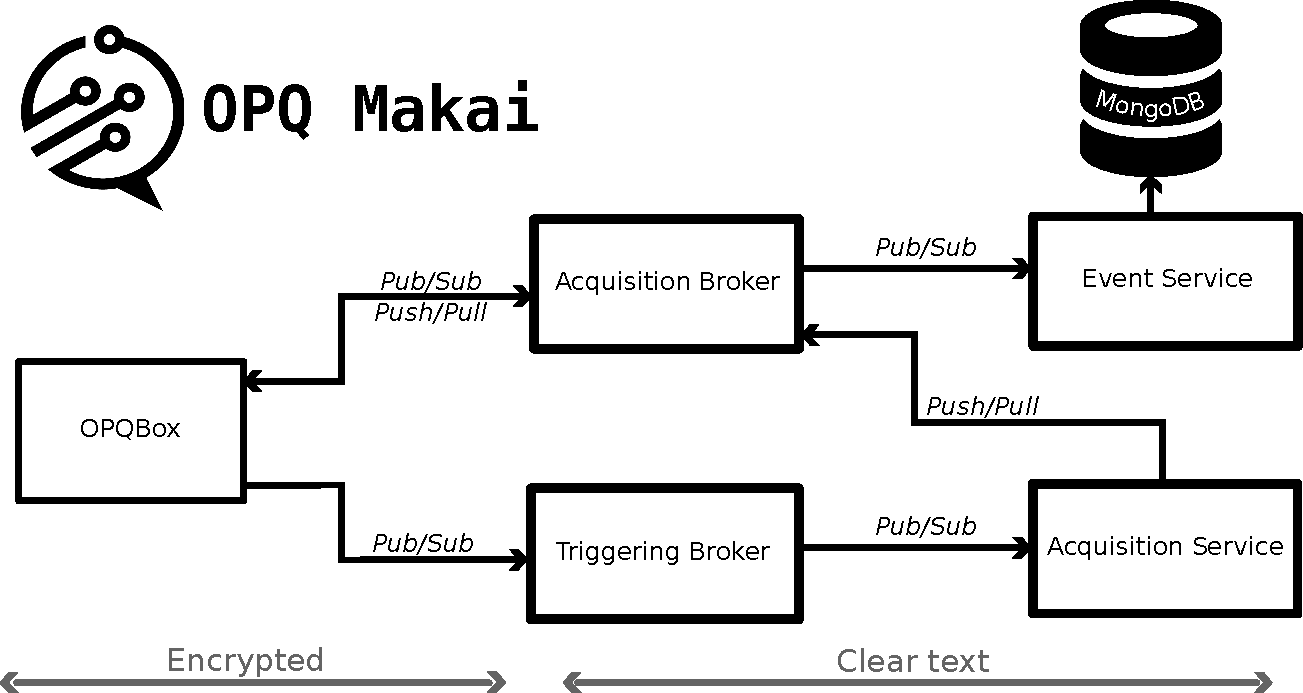
\includegraphics[width=3in]{images/makai/makai_main.pdf}
\caption{Makai component design}
\label{fig:makai-design}
\end{figure}

The Triggering Broker is perhaps the simplest component of the OPQ Makai system. The triggering stream generated by the OPQ Boxes is encrypted to preserve user privacy. In order to minimize the CPU time spent decrypting the data across multiple OPQ services, the Triggering Broker decrypts the data and sends clear text measurements to other OPQ cloud services. The Triggering Broker uses the ZeroMq subscribe socket to receive data from OPQ Boxes, and sends it via a publish socket to any connected client. Each publish message is published to a topic which corresponds to the ASCII representation of the originating OPQ Box ID. This allows services which utilize the Triggering Broker to select a subset of IDs to operate on. This is useful for load balancing the backend services, or dividing the OPQ network into separate regions with no electrical connections between them.

The Acquisition Broker manages the two-way communication between the OPQ Boxes and the rest of the cloud infrastructure. Unlike the triggering stream which originates from the OPQ Box, two-way communication is always initiated by OPQ cloud services. Two way communication is realized via a command response interface, where the OPQ service initiates the communication by sending a clear text command to the Acquisition Broker, which then forwards it in encrypted form to the appropriate OPQ Boxes.

The Acquisition Service resides between the Triggering and Acquisition Brokers. The Acquisition Service is responsible for three tasks:
(1) Computation of statistics of the incoming triggering stream; (2) Hosting plugins for triggering stream analysis; and (3) Generating data event requests for OPQ Boxes. The Acquisition Service accesses the triggering stream by connecting to the publish socket of the Triggering broker. Since the connection is managed through the ZeroMq publish-subscribe socket, several Acquisition Services can be connected to a single Triggering broker endpoint, each servicing a subset of OPQ Boxes by subscribing to only specific devices. The Acquisition Service does not include any analysis capabilities by default. Instead, analysis is performed by shared library loadable plugins. These plugins can be loaded and unloaded at runtime, thus allowing live upgrading and testing of new analysis methods.

The Event service is a microservice which stores raw data generated by OPQ Boxes in the MongoDB Database. On initialization, the Event service queries MongoDB database for the highest event number recorded so far, connects to the Acquisition Broker’s publish port, and subscribes to all messages that start with the prefix ``data”. This allows the Event service to capture every response from OPQ Boxes generated from commands issued by the Acquisition service plugins. Once the Event service receives a data response with an identity containing an event token it hasn’t seen before, it will increment the event number, and store it in an internal key value store.

\subsection{OPQ Mauka}
\label{sec:opq-mauka}

The previous sections discussed the design of OPQ Box, a custom hardware device for collecting four important measures of power quality, and OPQ Makai, a novel, hybrid centralized/decentralized data acquisition scheme which involves two-way communication between the OPQ Boxes.  As a result of these two innovations, an OPQ sensor network has the ability to collect and analyze high fidelity, low level data about power quality anomalies in a cost-effective, scalable fashion.

There are remaining challenges to creating a useful power quality sensor network. First, the data provided by OPQ Boxes is low-level, "primitive" data consisting of either features (i.e. frequency, voltage, THD, and transients) or waveform data. But what we actually want is actionable insights into grid stability. For example, we might want to know if a given anomalous data value is actually detrimental, or we might want to be able to predict when a power quality event might occur in the future based upon the recognition of cyclical events in the historical data.

A second challenge involves the potentially high volume of data might accumulate in the cloud. Although OPQ Box and OPQ Makai provide a scalable mechanism for communicating power quality data to the cloud services, it is still the case that, over time, a substantial amount of data could accumulate. One strategy is to simply store all of the data sent to the cloud forever. This means that data storage requirements will increase monotonically over time, making the sensor network more costly to maintain the longer it is in place. An alternative strategy is to implement an algorithm to identify uninteresting (or no longer interesting) data and discard it.  Ideally, such an algorithm would enable OPQ sensor network designers to calculate an upper bound on the total amount of cloud storage required as a function of the number of nodes (OPQ Boxes) in the network.

OPQ Mauka addresses both of these issues. First, OPQ Mauka provides a multi-layered representation for structuring and processing DSN data. The structure and processing at each layer is designed with the explicit goal of turning low-level data into actionable insights. Second, each layer in the framework implements a "time-to-live" (TTL) strategy for data within the level. This strategy states that data must either progress upwards through the layers towards more abstract, useful representations within a fixed time window, or else it can be discarded. The TTL strategy is useful because when implemented, it allows DSN designers to make reasonable predictions of the upper bounds on data storage at each level of the framework adjusting for the number of sensors and power anomaly probability.

 TTL also makes possible a ``graceful degradation" of system performance if those bounds turn out to be exceeded. For example, consider a situation in which a power network enters a prolonged period of widespread power quality instability, where every OPQ Box is reporting continuous anomalous conditions with respect to voltage, frequency, THD, and transients.  This ``worst case scenario" would lead to the potential situation of every OPQ Box trying to upload raw waveform data all the time. The TTL system provides safeguards, in that whatever low-level data has not been processed relatively quickly can be discarded.  Thus, instead of the system potentially going down entirely, it could instead continue to operate at a reduced capacity.

Figure \ref{fig:mauka-data-model} illustrates the hierarchical data model for OPQ Mauka. This data model can be conceptualized as a multi-level hierarchy that adaptively optimizes data storage using a tiered TTL approach and provides a mechanism in which typed aggregated data is continually refined to the point of being of becoming actionable. The data model also includes software components called "actors" that both move data upward through the levels and also apply optimizations downward through the levels. Actors are implemented through a plugin architecture, making it easy to experiment with the data model and improve it over time.

\begin{figure}
\center 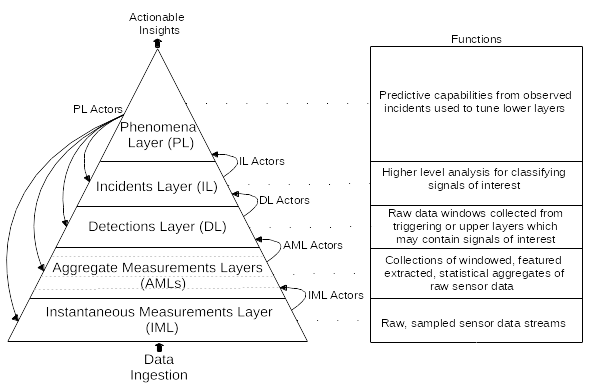
\includegraphics[width=4in]{images/mauka/mauka-data-model.png}
\caption{Mauka data model hierarchy}
\label{fig:mauka-data-model}
\end{figure}

The lowest layer of the hierarchy is the Instantaneous Measurements Layer (IML). The IML contains "raw" data, in other words, the digitized waveform.  IML data exists both on each OPQ Box (where it is available for up to the previous 60 minutes). It also exists in the cloud, in the event that OPQ's triggering mechanism has caused a temporal interval of waveform data to be uploaded. IML data in the cloud has a TTL of 15 minutes: unless the waveform data is found to be useful by a cloud service within 15 minutes, it can be discarded.

The second layer is the Aggregate Measurements Level (AML). The AML stores power quality summary statistics sent either once per second or once per minute by each OPQ Box. These summary statistics include the maximum, minimum, and average values of voltage, frequency, THD, and transient metrics over the time window. It is AML data that is used to initiate the triggering process of uploading IML data from the cloud.

The third layer is the Detections Level (DL). This layer is responsible for processing the IML and AML data to produce a representation of an "event" with a precisely defined start and end time based upon examination of the waveform.  As will be discussed in Section \ref{sec:subthreshold-events}, knowledge of the start and end time of a power quality anomaly allows investigation of how that anomaly might manifest itself elsewhere in the grid, even if this manifestation is not severe enough to produce over-threshold data values.

The fourth layer is the Incident Level (IL).  This layer starts to answer the question of whether the data is "actionable" by classifying the detected event according to various industry standards for power quality anomalies: IEEE 1159, ITIC, SEMI F47, and so forth.  For example, an event that falls into the ITIC "prohibited" region clearly indicates a power quality anomaly that requires further study and intervention.

The fifth and final level is the Phenomena Level (PL). This layer contains the results of analyses that attempt to identify cyclic, and thus predictable, power quality disturbances. It also contains analysis results regarding the similarity of various incidents, which can help uncover causal factors.  Finally, it provides analyses for adaptive optimization of the OPQ Sensor Network. These optimizations can change the thresholds for individual boxes to either increase their sensitivity or decrease their sensitivity over specific intervals of time. The ultimate goal of adaptive optimization is to help the network learn to acquire all of the data useful for analyses, and only the data useful for analyses.  We are still in the early stages of exploring the potential of adaptive optimization in OPQ networks.

\subsubsection{OPQ Mauka: Actors}

The current capabilities of OPQ Mauka can be summarized in terms of its Actors, which are implemented as plugins. Nine of the most important Actors are described below.

{\em Makai Event Actor.} The Makai Event Actor is responsible for reading data newly created by OPQ Makai into OPQ Mauka. It performs feature extraction on the raw data stream and forwards those features (or the raw data) to subscribing Actor plugins. This allows OPQ Mauka to perform feature extraction once, and allow use of those features by multiple Actors.

{\em Frequency Variation Actor.} The Frequency Variation Actor classifies generic frequency sags, swells, and interruptions as defined by the IEEE 1159 standard. Both duration and deviation from nominal are used to perform these classifications. Duration classifications include frequency deviations that last for less than 50 ns, between 50 ns to 1 ms, and 1 ms to 50 ms. Classifications for deviations from nominal are performed for values that are up to 40\% deviation from nominal. This Actor is able to classify frequency swells, frequency interruptions, and frequency sags, leading to the creation of data at the Incident Layer.

{\em IEEE 1159 Voltage Actor.} The IEEE 1159 Voltage Actor is used to classify voltage Incidents in accordance with the IEEE 1159 standard[29]. In general, this standard classifies voltage disturbances by duration and by magnitude. Voltage durations are classified from 0.5 to 30 cycles, 30 cycles to 3 seconds, 3 seconds to a minute, and greater than 1 minute. Voltage deviations are classified in both the sag and swell directions as a percentage from nominal. Sags are generally classified between 10\% and 90\% of nominal while swells are generally classified from 110\% to 180\% of nominal. This Actor is capable of classifying voltage sags, swells, and interruptions as defined by the standard, and creating data at the Incident Layer if appropriate.

{\em Box Optimization Actor.} The Box Optimization Actor is responsible for sending and receiving typed messages to and from OPQ Boxes from OPQ Mauka. This Actor is capable of requesting the state of each OPQ Box (e.g. uptime, Measurement rate, security keys, etc). It is also capable of adjusting the state of individual OPQ Boxes by changing things such as the Measurement and Trend rate or the sampling rate used by the Box.

{\em Future Phenomena Actor.} The Future Phenomena Actor is responsible for creating Future or Predictive Phenomena. These Phenomena are used to predict Events and Incidents that may occur in the future. This plugin does not subscribe to any messages, but instead utilizes timers to perform its work. By default, this plugin runs every 10 minutes.

When a Future Phenomena Actor runs, it loads any active Periodic Phenomena found in the database. If Periodic Phenomena are found, this Actor extrapolates possible Detection and Incident Layer data by first examining their timestamps and then extrapolating into the future using the mean period and the standard deviation. For each timestamp in a Periodic Phenomena, the mean period is added. If the resulting timestamp is in the future, a Future Phenomena is created using the time range of the future timestamp plus or minus the standard deviation of the Periodic Phenomena.

When a Future Phenomena is created, timers are started in a separate thread signifying the start and end timestamps of the Future Phenomena. When the first timer runs, messages are sent to the Box Optimization Actor and the Threshold Optimization Actor instructing OPQ Box thresholds to be set lower and measurement rates to be set higher. This increases the chance of seeing an anomaly over the predicted time window. When the second timer runs, these values are reset to their default values. Thus, the plugin increases fidelity and decreases thresholds over the period of a Future Phenomena.

{\em ITIC Actor.} The ITIC Actor analyzes voltage to determine where it falls within the ITIC curve \cite{thallam_power_2000}. The ITIC curve is a power acceptability curve that plots time on the x-axis and voltage on the y-axis.  The purpose of the curve is to provide a tolerance envelope for single-phase 120V equipment. The curve defines three regions. The first region is "No Interruption" and generally includes all voltages with very short sustained durations. All events within this region have no noticeable effect on power equipment. The second region, the "No Damage Region", occurs during voltage sags for extended periods of time. Power Events in this region may cause equipment interruptions, but it will not damage the equipment. The final region, the "Prohibited" region, is caused by sustained voltage swells and may cause damage to power equipment. This Actor determines if an event falls within the "No Damage" or "Prohibited" regions and if so, creates an Incident to record this.

{\em SEMI F47 Actor.} The SEMI F47 Actor is similar to the ITIC Actor in that it plots voltage and duration against a power acceptability curve. In this case, the standard used is the SEMI F47 standard \cite{djokic_sensitivity_2005}. Rather than using a point-in-polygon approach, this plugin reads the voltage features sequentially and uses a state machine to keep track of the current classification. This plugin only classifies values as a "violation" or as "nominal".

{\em Transient Actor.} The Transient Actor is responsible for classifying frequency transients in power waveforms. The plugin subscribes to messages from a topic which contains a calibrated power waveform payload. The Transient Actor is capable of classifying impulsive, arcing, oscillatory, and periodic notching transients. A decision tree is utilized to select the most likely transient type and then further analysis is used to perform the actual classification of transients. Dickens et al \cite{dickens_transient_2019} provides more details on the transient classification system used by this Actor.

{\em Periodicity Actor.} The Periodicity Actor is responsible for detecting periodic signals in power data. This Actor does not subscribe to any messages, but instead runs off of a configurable timer. The Actor is set to run by default once an hour and every hour it scrapes the last 24 hours worth of data and attempts to find periods in the Measurements over that duration.

For each feature in the Measurement and Trend data (e.g. frequency, voltage, and THD), the Periodicity Actor first removes the DC offset from the data by subtracting the mean. Next, the Actor filters the signal using a 4th order high-pass filter to filter out noise. The Actor then performs autocorrelation on the signal followed by finding the peaks of the autocorrelation. The mean distance between the peaks of the autocorrelation provides the period of the signal.

The Periodicity Actor only classifies data as periodic if at least 3 peaks were found and the standard deviation of the period is less than 600 seconds (10 minutes). Once a positive identification has been made, peak detection is performed on the original signal. Once the plugin has the timestamps and deviations from nominal of the periodic signal of interest, the plugin can group Measurements, Trends, Detection Layer Events, and Incidents that were created during the periodic signals together as part of the Periodic Phenomena.

\subsection{OPQ View}
\label{sec:opq-view}

The final component of the OPQ Sensor Network system architecture is called OPQ View. It is a web application, implemented using the Meteor application framework, which provides a variety of visualization and query services.  An example of the OPQ View home page is provided in Figure \ref{fig:opq-view-home}.

\begin{figure}
\center 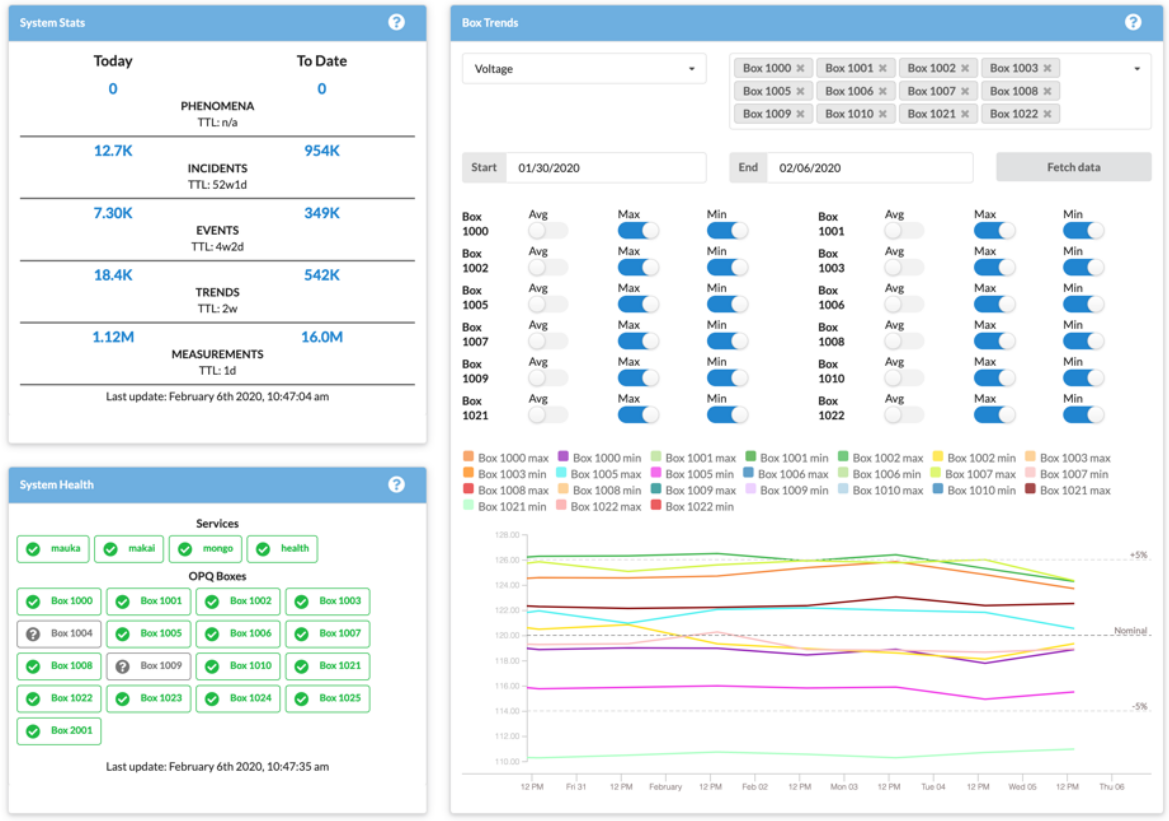
\includegraphics[width=5in]{images/view/homepage.png}
\caption{OPQ View: home page}
\label{fig:opq-view-home}
\end{figure}

The home page provides three components:  a "System Stats" window which indicates the number of data elements currently at each level of the OPQ Mauka data hierarchy, a "System Health" window that indicates whether the Cloud services appear to be running correctly and the status of communication with all known OPQ Boxes on the sensor network, and a "Box Trends" visualization that provides the ability to quickly see trends in the four basic measures (Voltage, Frequency, THD, and Transients) over time.

Figure \ref{fig:opq-view-box-map} shows a map-based view of the sensor network. This figure shows the location of 11 OPQ Boxes on the University of Hawaii campus at one point during Fall of 2019. Depending on the zoom level of the interface, some boxes are collapsed into disks with a number indicating the number of boxes at that location. Zooming in reveals more information about the box including near-real time values for voltage and frequency, as is shown for the box in the upper right corner of the figure.

\begin{figure}
\center 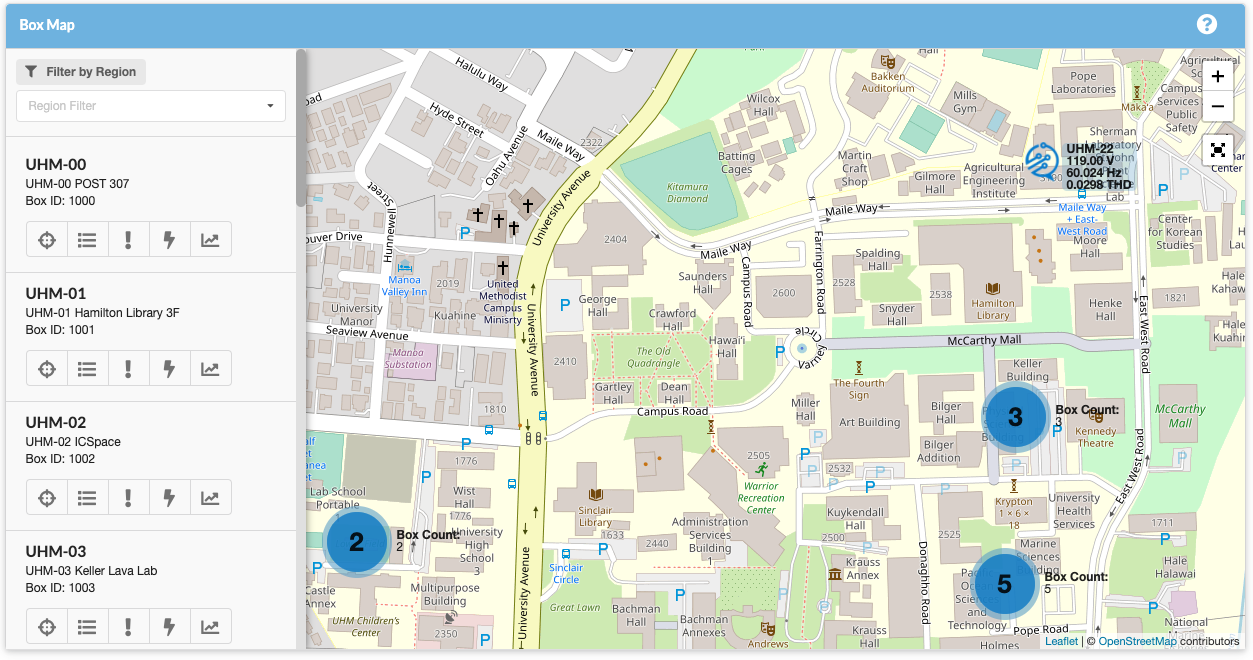
\includegraphics[width=5in]{images/view/boxmap-2.png}
\caption{OPQ View: Box Map}
\label{fig:opq-view-box-map}
\end{figure}

Figure \ref{fig:opq-view-incident-summary} shows a visual display of a single Incident. This view includes a map-based location of the box whose data was involved in the Incident, the start and end time and duration of the Incident, the classification(s) of the anomalous data, and the waveform associated with the Incident (when applicable). If additional analysis is desired, the raw data can be downloaded in CSV format.

\begin{figure}
\center 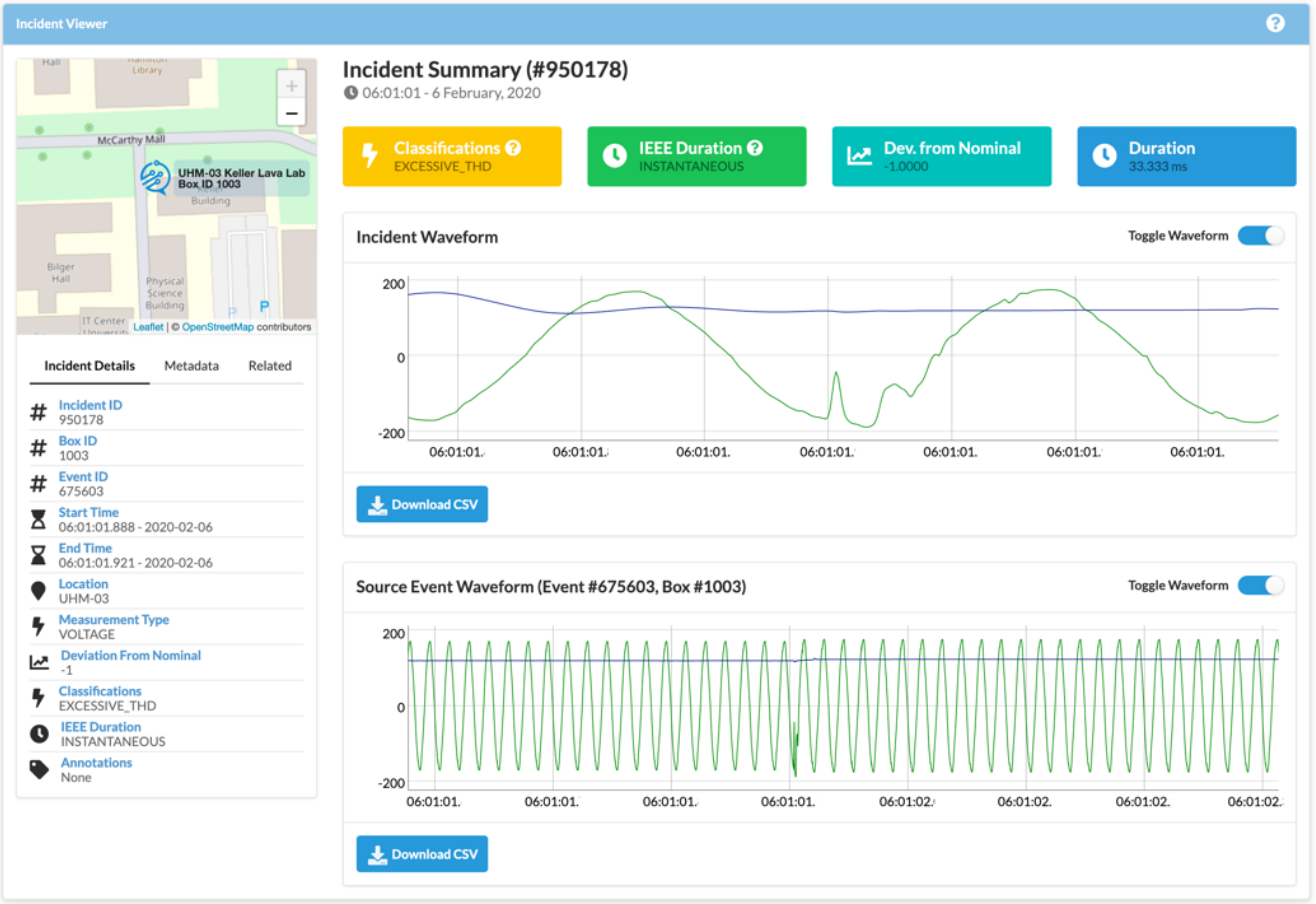
\includegraphics[width=5in]{images/view/incident-summary.png}
\caption{OPQ View: Incident Summary}
\label{fig:opq-view-incident-summary}
\end{figure}

The above images provide a sense for how OPQ View helps users to understand, monitor, and assess an OPQ Sensor Network and the underlying power quality of the grid it is attached to. There are several features in OPQ View for user and box management; for details, please see the OPQ View documentation.

While OPQ View provides a variety of useful visualization and analysis features, users wishing to understand the power quality of their grid are not restricted to its current feature set. The OPQ database schema is public, and if a new analysis is desired, it is straightforward to query the database directly for the data of interest and build a new analysis off of it.



















\section{Related Work}
\label{sec:related-work}

This section explains how OPQ fits into current industry solutions as well as academic research on power quality monitoring and analysis. For the purposes of this review, we exclude utility-side power quality monitoring and analysis systems.

\subsection{Power quality hardware}
\label{sec:commercial-pq-devices}

There exists a very wide variety of power quality hardware devices, including those made by Fluke \cite{fluke_fluke_2020}, Dranetz \cite{dranetz_dranetz_2020}, Elspec \cite{elspec_elspec_2020}, PowerSide (formerly Power Standards Lab) \cite{powerside_powerside_2020}, ACR Systems \cite{acr_acr_2020}, and OpenZMeter \cite{viciana_openzmeter_2018}.

All of the above devices contrast with the OPQ Box in similar ways. First, all of them collect a wider variety of power quality measures than OPQ Box, and most have been certified according to one or more industry standards. Except for OpenZMeter, they are generally designed to support industrial applications, where the goal is to ensure that the power being supplied to a building or plant is of adequate quality, and/or that the machinery in the plant is not degrading power quality. Apart from the PowerWatch monitor, all of them are attached to electrical mains using current transformers. Finally, all of them are designed for "stand alone" operation: each device can independently gather and assess power data.

While the OPQ Box has much more limited functionality, it is designed to be manufactured for approximately \$75, which is 10 to 100 times less expensive than most commercial devices, and similar is cost to OpenZMeter. The most important distinguishing feature of OPQ Box is that it is designed to grid-level, not single point monitoring, and thus incorporates features (such as two-way communication with the cloud, and subthreshold triggering) that are not present in devices intended for "stand alone" capabilities.

\subsection{Power quality software}
\label{sec:commercial-pq-software}

PQView \cite{electrotek_concepts_pqview_2020},  PQSCADA Sapphire \cite{elspec_ltd_pqscada_2016}, PQDIF \cite{sabin_ieee_2020}, and Grid Protection Alliance \cite{grid_protection_alliance_grid_2020}  are examples of software and/or software standards for manipulating power quality data.

The differences between the way OPQ and the above systems store and manipulate power quality data arise from fundamentally different architectural assumptions and the historical background of the technology. PQView and PQSCADA Sapphire are designed to operate in a technology environment consisting of a large number of installed, "stand alone" power quality monitors built by different vendors. Their goal is to aggregate the data collected by these devices, and in order to do so, they depend upon the PQDif standard as a way to obtain power quality data independent of the vendor and device generating it. This results in a kind of "store and forward" process: power quality data is captured and stored on the device, and then periodically bundled into a PQDif file and sent to the database software.

OPQ Cloud, on the other hand, is designed only to support the capabilities of OPQ Boxes. OPQ Boxes, furthermore, have no "stand-alone" capability; they maintain continuous connection to the Internet and upload power quality data to cloud-based services as needed. This means that OPQ implements a very different approach to representing and transmitting data than PQDif. For details on the representation, see the OPQ Data Model, and for details on communication, see the OPQ Protobuf protocol.

\subsection{Research systems}

Di Manno et al \cite{di_manno_user_2015} describes a PQ monitoring system called PiKu. Unlike OPQ, PiKu is designed as a hardware device for sensing power quality that is directly integrated into a PC. Systems with similar architectures include TRANSIENTMETER, described in Da Ponte et al \cite{daponte_transientmeter:_2000}, BK-ELCOM, described in Bilik et al \cite{bilik_modular_2007}, and a system described in Xu et al \cite{xu_distributed_2012}.

There are also research projects based upon leveraging existing monitoring infrastructure. Suslov et al \cite{suslov_distributed_2014} describes a distributed power quality monitoring system based upon existing phasor measurement units installed by utilities. Sayied et al \cite{sayied_power_2013} describes a system designed using existing smart meters. Kucuk et al \cite{kucuk_extensible_2010} describes a similar system for the Turkish National Grid using utility grid monitoring infrastructure.

Mohsenian-Rad et al. \cite{mohsenian-rad_distribution_2018} designed the $\mu$PMU (phase measurement unit) system which provides distributed power quality measurements over power grid distribution systems. The $\mu$PMUs in conjunction with their backend software provide two types of analytics. Descriptive analytics provide information about the types and classifications of power quality issues that are observed within the power distribution grid. Predictive analytics are used to predict future power quality issues. The authors describe their system as providing the ground for for enabling future prescriptive analytics, which is the idea of self-tuning the DSN to prepare for future power quality problems by using a combination of descriptive and predictive analytics. In contrast, as we will discuss in Section \ref{sec:adaptive-optimization}, the OPQ sensor network already supports self-tuning through adaptive optimization.

One research system very similar in spirit to OPQ is FNET \cite{liu_distribution_2017}. Like OPQ, the FNET system consists of custom hardware that monitors the electrical signal from a wall outlet, and uploads data to the cloud for further processing. Unlike OPQ, FNET is designed for monitoring of frequency disturbances, how they propagate across wide area (i.e. nation-wide) utility grids, and, if possible, where the frequency disturbance originated. This means that FNET devices must be synchronized using GPS, and that the data collected consists of frequency and voltage angle. OPQ is designed for more "local" grid analysis, and we are not interested in propagation. As a result, OPQ Boxes are synchronized using NTP rather than GPS, which reduces cost and simplifies installation (OPQ Boxes do not need line of site to a GPS satellite). Finally, FNET hardware appears to support only "one way" communication from device to the cloud, while OPQ Boxes support "two way" communication (from box to cloud, and from cloud to box).

\section{Results and Discussion}
\label{sec:pilot-study}

To evaluate the capabilities of the OPQ Sensor Network, we deployed 16 OPQ Boxes at the University of Hawaii Manoa campus over the course of three months in the Fall of 2019.  The University of Hawaii campus is an isolated microgrid connected to the Oahu powergrid only via a single 46kV feeder. The UH Campus also has commercial electrical meters (a mixture of GE PQMII and GE EPM 7000) deployed across various levels of the power delivery infrastructure. While the primary purpose of these meters is to monitor power consumption, they do include power quality monitoring capabilities. Data from these meters were used as ground truth for validation studies of the OPQ sensor network.

Our pilot study is significant because much of the literature on power quality assessment relies on models, not actual installations \cite{anurangi_effects_2017,bayindir_effects_2016,farhoodnea_power_2012,shafiullah_experimental_2014}. In other cases, data was collected from only one location or for a very short time span \cite{kucuk_assessment_2013,viciana_openzmeter_2018}.

\subsection{Descriptive statistics}

The pilot study started on October 7, 2019 and ended on February 4, 2020. We deployed 16 OPQ Boxes across campus. As noted above, each OPQ Box collects 200 measurements per grid cycle, for a total of approximately 1B raw measurements per day per box.  Values for the maximum and minimum voltage, frequency, and THD, along with the presence or absence of transients, is sent once a second to the cloud by each box. Thus, each box sends approximately 86,400 measures per day to the cloud at a minimum. Over the course of the pilot study, a total of approximately 116M aggregate measures were sent by all of the OPQ Boxes.

Figure \ref{fig:statistics} provides two additional sets of summary statistics regarding the pilot study.  Figure (a) shows the number of anomalous events (i.e. where threshold values for frequency, voltage, THD, or transients were exceeded) along with the number of OPQ Boxes that experienced the power quality anomaly during that same time period. So, for example, 170,925 power quality anomalies were experienced by only one of the 16 OPQ boxes, and 463 anomalous power quality measurements were experienced by all 16 OPQ Boxes.

\begin{figure}[ht]
	\centering
	\begin{subfigure}{.5\textwidth}
        \begin{tabularx}{\textwidth}{XXXX|}
            \toprule
            \textbf{Events} & \textbf{Boxes} & \textbf{Events} & \textbf{Boxes} \\
            \midrule
            170,925 & 1 & 203 & 9 \\
            1,654 & 2 & 160 & 10 \\
            1,109 & 3 & 162 & 11 \\
            853 & 4 & 130 & 12 \\
            593 & 5 & 169 & 13 \\
            416 & 6 & 210 & 14 \\
            354 & 7 & 477 & 15 \\
            246 & 8 & 463 & 16 \\
             &  &  &  \\
            \bottomrule
        \end{tabularx}
	  \caption{Summary statistics: Events}
	\end{subfigure}%
	\begin{subfigure}{.5\textwidth}
	 \begin{tabularx}{\textwidth}{lX}
               \toprule
               \textbf{Incident} & \textbf{Total}  \\
               \midrule
               Frequency Swell & 291,235 \\
               Frequency Sag & 244,286  \\
               Excessive THD & 21,395 \\
               Voltage Sag & 620 \\
               ITIC (No Damage) & 93 \\
               SEMI F47 (Violation) & 24 \\
               Voltage Interruption & 16 \\
               Frequency Interruption & 14 \\
               Voltage Swell & 8 \\
               \bottomrule
           \end{tabularx}
   	  \caption{Summary statistics: Incidents}
	\end{subfigure}
	\caption{Summary statistics of (a) boxes involved in events and (b) incident type occurrences}
	\label{fig:statistics}
\end{figure}

\subsection{OPQ provides valid and reliable collection of power quality data}
\label{hyp:01}

The first goal of the pilot study was to assess how well an OPQ sensor network is able to collect basic power quality data. To do this, we compared data on voltage and frequency collected by OPQ Boxes with data on voltage and frequency collected by the existing UH power monitors.  The results are shown in Figure \ref{fig:opqbox-f-v-validation}.

\begin{figure}[ht]
	\centering
	\begin{subfigure}{.5\textwidth}
	  \centering
	  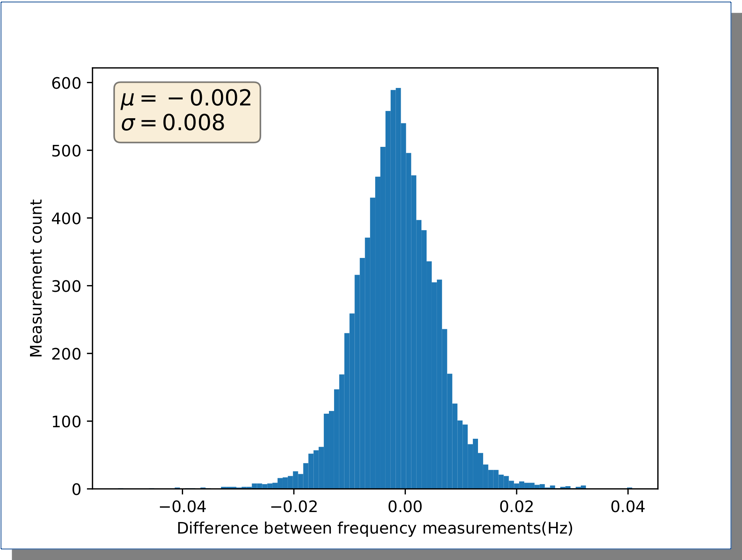
\includegraphics[width=0.9\linewidth]{images/pilot/opqbox-frequency-validation.png}
	  \caption{Frequency differences}
	  \label{fig:opqbox-validation-1}
	\end{subfigure}%
	\begin{subfigure}{.5\textwidth}
	  \centering
	  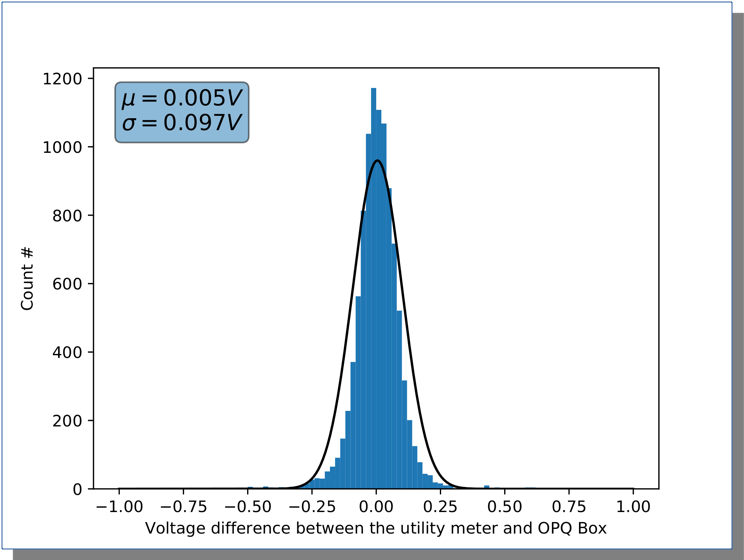
\includegraphics[width=0.9\linewidth]{images/pilot/opqbox-voltage-validation.png}
	  \caption{Voltage differences}
	  \label{fig:opqbox-validation-2}
	\end{subfigure}
	\caption{Validation of (a) Frequency and (b) Voltage}
	\label{fig:opqbox-f-v-validation}
\end{figure}

As the charts illustrate, there is very close correspondence between the building meters and the OPQ Boxes. For frequency differences, the value of $\sigma$ is 0.0079 Hz, and for voltage, $\sigma$ is 0.1703 V. (Note that typical thresholds for frequency and voltage PQ anomalies is 1 Hz and 6 V, so OPQ Box values appear accurate enough for their intended purpose.)

Validating THD and transient data, the other two basic power quality measures collected by OPQ Boxes, was more challenging.

Figure \ref{fig:opqbox-thd-validation} shows the results of comparing values of THD collected by OPQ Boxes and building meters.

\begin{figure}[ht]
  \centering
	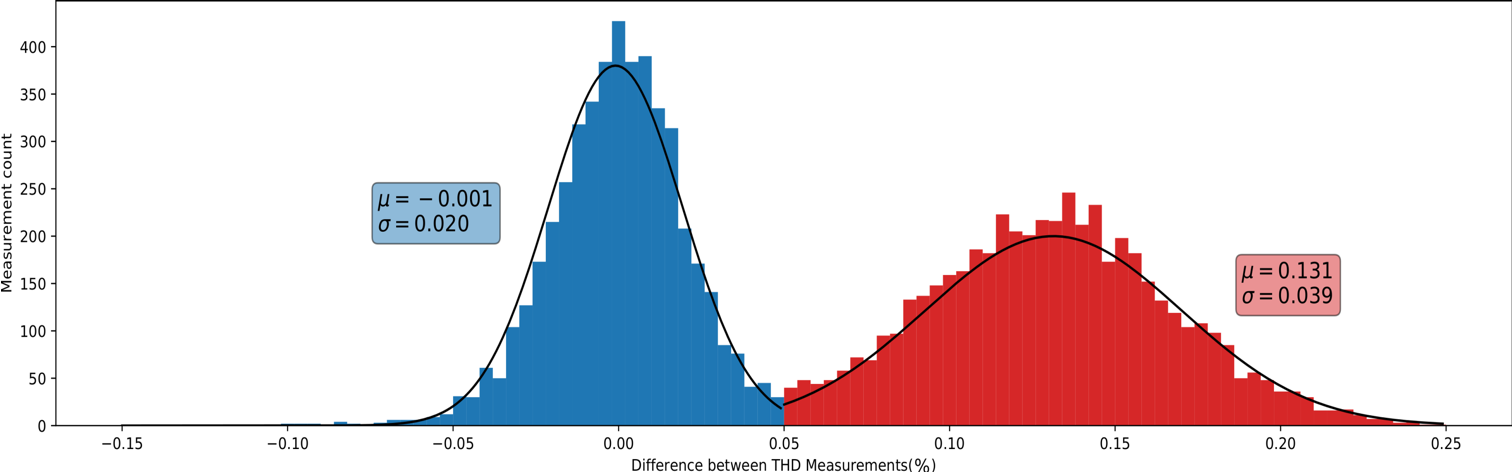
\includegraphics[width=0.8\linewidth]{images/pilot/opqbox-thd-validation.png}
	\caption{THD differences}
	\label{fig:opqbox-thd-validation}
\end{figure}

During the hours of 6pm and 6am, OPQBox and the building level meter displayed a high level of agreement as shown in the blue histogram in Figure \ref{fig:opqbox-thd-validation}.
On the other hand, during the hours of 6pm and 6am, there was a static disparity of 0.13\% between the two meters as portrayed  in the red histogram.
This is likely attributed to the meter location in the power transmission hierarchy.
While the OPQ Box is plugged the $120V_{ac}$ line, the building meter is monitoring the $480V_{ac}$ three phase line.
An additional active conditioning system installed along side the transformer responsible for compensating for reactive power in the building is the likely culprit in the disparity.

Unfortunately, we unable to perform validation of transient data collection, because building meters did not provide us with access to that information.
However, synthetic tests performed in the lab against a calibration source, showed that OPQ Box is able to measure transient magnitude with $\sigma=0.125V$, significantly higher then the triggering threshold.
It should be noted that the internal transient metric provided by the OPQ Box is only used for event detection, while higher level analytics compute their own transient classification parameters.
As such, the transient detection capabilities of the OPQ Box are more than sufficient for its role in the OPQ ecosystem.

\subsection{OPQs triggering system provides advantages with respect to bandwidth and computation}
\label{hyp:02}

The pilot study provided an opportunity to collect data on the resources required by an OPQ sensor network with respect to cloud-level network resources and server-level computation overhead.

To assess network bandwidth utilization, we analyzed the data stream of frequency and voltage collected by OPQ Boxes, and the resulting network bandwidth utilized by the OPQ Makai triggering algorithm. Over the course of a typical day, OPQ Makai requested approximately 136 MB of data from the deployed OPQ Boxes.  We then calculated how much data would be sent by a power quality meter using more conventional triggering approach in which exceeding a threshold would automatically result in sending waveform data, and found that, under the same conditions, approximately 1025 MB would be sent to the cloud, or eight times the network bandwidth.

The computational cost of an OPQ sensor network is proportional to the amount of data acquired. Since the meter level analytics are at best only good enough for event detection, further analysis is required for event classification.
This implies that the OPQ Makai triggering algorithm is at least 8 times more efficient then the self triggered counterpart, since 8 times less data is sent by OPQ Boxes to the cloud for analysis.

\subsection{OPQ enables subthreshold event detection based on temporal locality}
\label{sec:subthreshold-events}

One interesting capability enabled by two-way communication between OPQ Boxes and their cloud-based services is what we term {\em subthreshold event detection based on temporal locality}.
In a nutshell, when one OPQ Box determines that a power quality measure has exceeded a threshold, one of the actions of the sensor network is to request high fidelity waveform data from neighboring boxes for the same temporal period, regardless of whether those boxes are reporting over-threshold data.
In the event that any of those boxes actually do report over-threshold data, then the request ripples outward to the boxes neighboring that box, and so forth.
This is accomplished by maintaining a model of the OPQ Box metrics for each device.
Once a single device passes a threshold, OPQ Makai will search the network for all other devices which exhibit measurements which deviate significantly from the device model.
If more devices are located, data from all the affected devices will be captured.
Otherwise, the event is deemed local and ignored.

Sub-threshold triggering allows for clustering of OPQ Boxes based on their electrical distance without a priori knowledge of the power grid topology.
A distance metric comprised of the magnitude of the $V_{rms}$  disturbance between every pair of OPQ Boxes was used as the clustering parameter.
This distance metric describes how much local disturbances observed by a device affect every other device on the network.
Hierarchical clustering employed on the aforementioned distance metric results in the hierarchy shown in Figure \ref{fig:clustering}.
These clusters closely corresponded to the topology of the power grid.
For example the two top-level clusters correspond to the two 12kV feeders which power the university campus.
As such, disturbances which originate on one feeder, have a minimal impact on the other.
On the other hand, devices 1009 and 1008 are located in adjacent buildings, and a common 480V feeder, resulting in large level of commonality in observed anomalies.
Sub-threshold triggering along with clustering in turn made it possible to perform limited localization of PQ incidents without prior knowledge of the grid layout.
In example, consider a $V_{rms}$ sag observed by the OPQ network shown in Figure \ref{fig:localisation}.
This event had the largest impact on devices 1008 and 1009 which as shown via hierarchical clustering are closely coupled.
From this information it is possible to conclude that the event depicted in Figure \ref{fig:localisation} originated from inside the UH power grid relatively close to devices 1008 and 1009.

\begin{figure}[ht]

    \centering
    \begin{subfigure}{.5\textwidth}
        \centering
        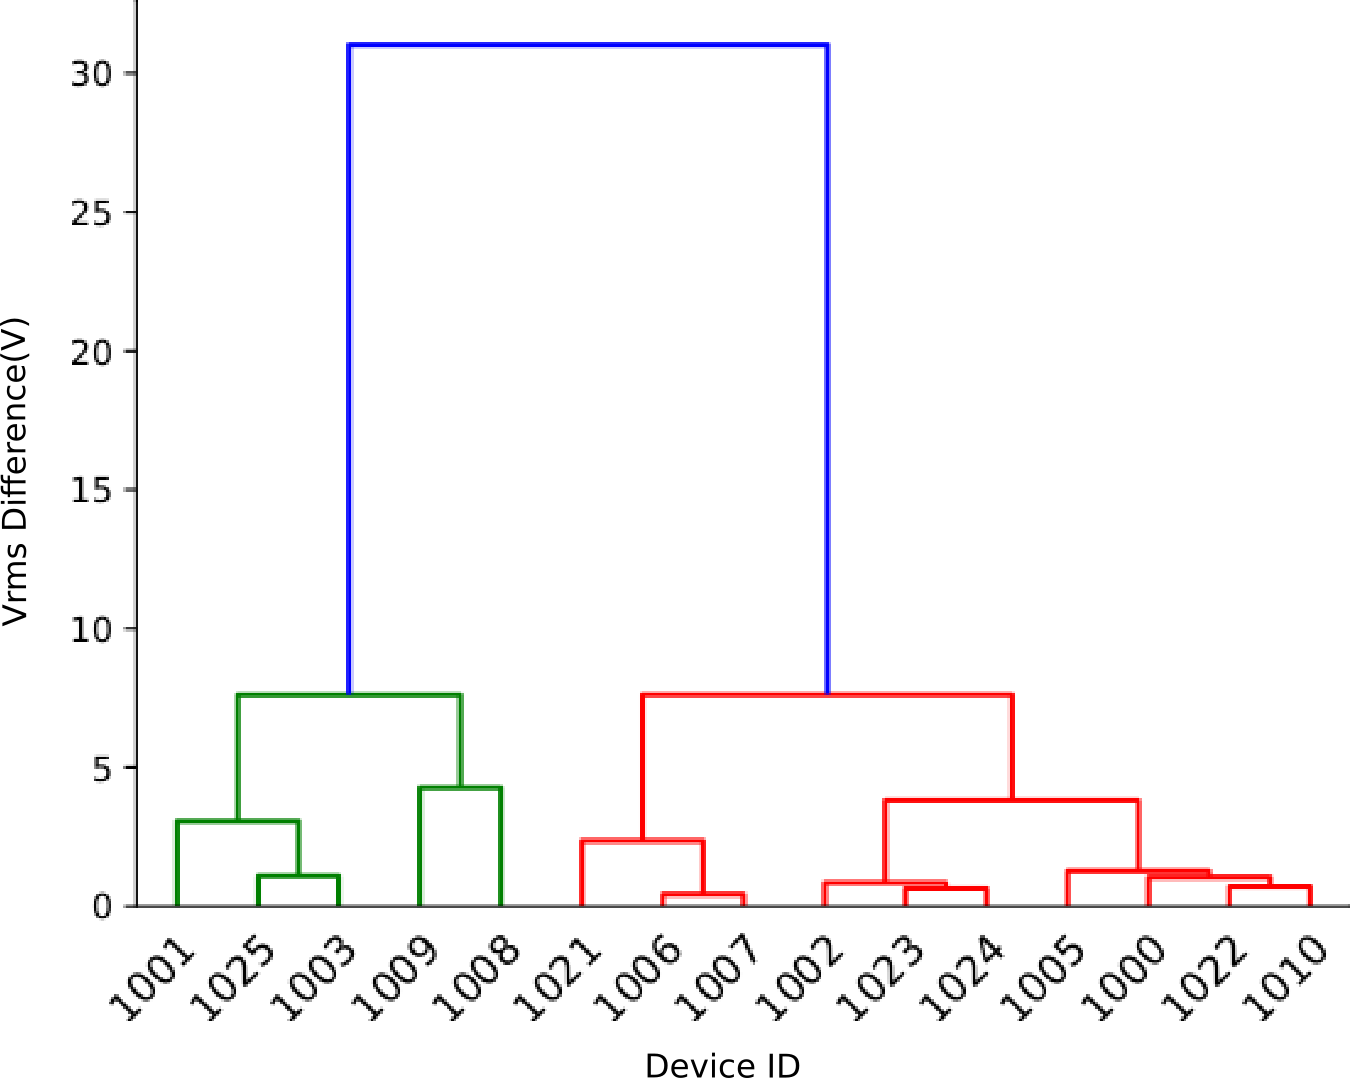
\includegraphics[width=0.9\linewidth]{images/pilot/clustring.png}
        \caption{Hierarchical clustering of OPQ Boxes.}
        \label{fig:clustering}
    \end{subfigure}%
    \begin{subfigure}{.5\textwidth}
        \centering
        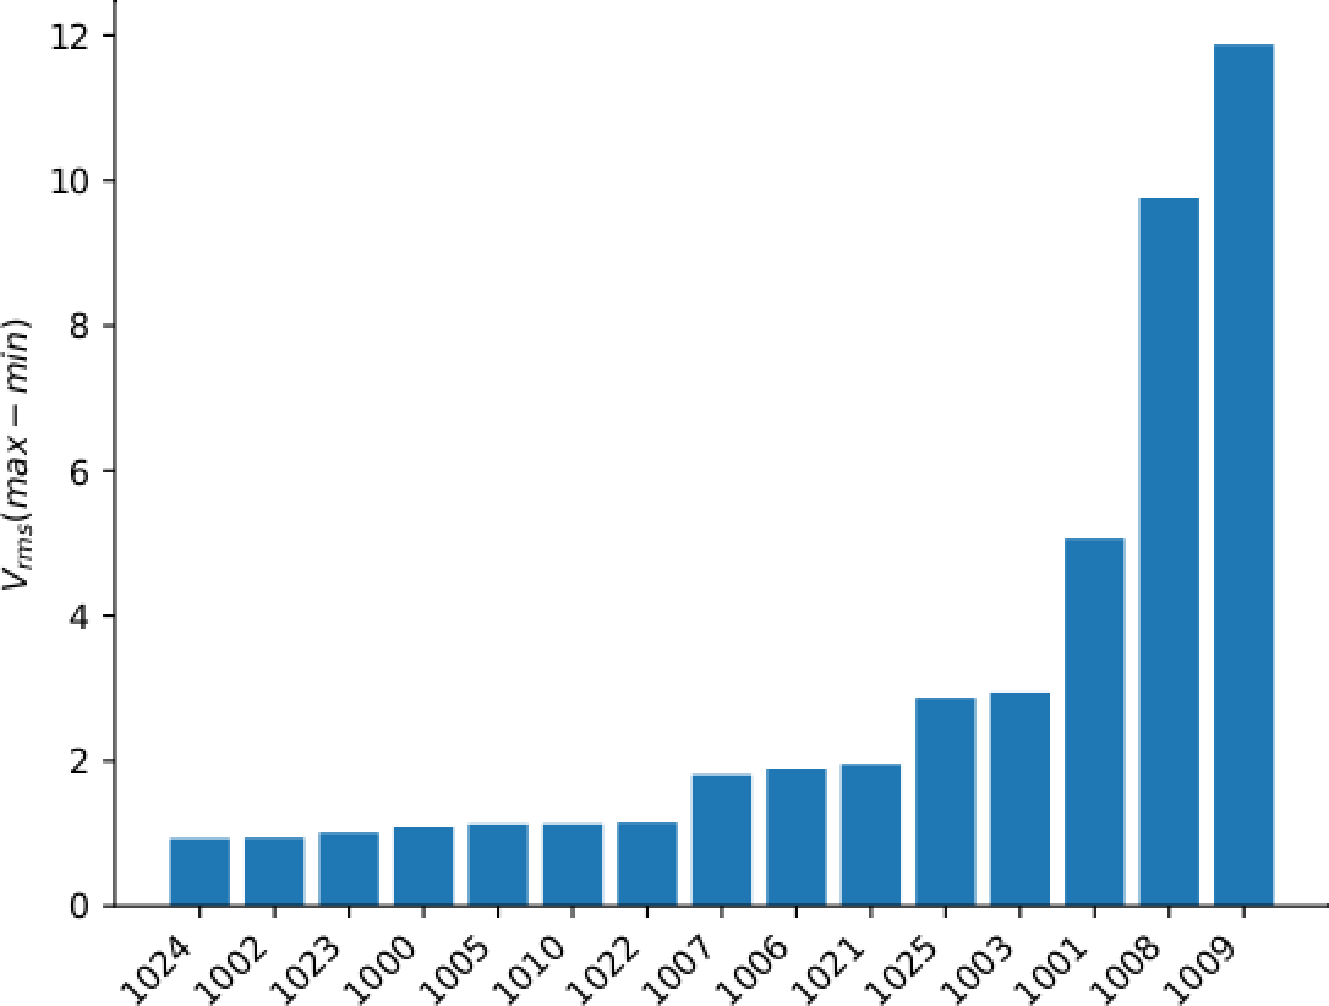
\includegraphics[width=0.9\linewidth]{images/pilot/localisation.png}
        \caption{Localisation of a disturbance.}
        \label{fig:localisation}
    \end{subfigure}
    \caption{Hierarchical clustering of OPQ Boxes, and localization of a disturbance.}
    \label{fig:localization-clustering}
\end{figure}

\subsection{The OPQ Information Architecture provides a means to produce actionable insights}
\label{hyp:04}

Figure \ref{fig:level-statistics} provides some descriptive statistics on the total number of entities created at each layer of the OPQ Information Architecture over the course of the pilot study. Note that the number of entities at a given layer at a given point in time is typically far less, due to the use of TTL to discard entities not promoted to higher layers.

\begin{figure}[ht]
  \centering
		 \begin{tabularx}{.4\textwidth}{lX}
       \toprule
       \textbf{Level} & \textbf{Total}  \\
       \midrule
       Phenomena & 10.4K \\
       Incidents & 415K \\
       Detections & 91.4K \\
       AML (Trends) & 1.94M \\
       AML (Measurements) & 116 M \\
       IML  & 100B \\
       \bottomrule
     \end{tabularx}
	\caption{Entities created at each level of the OPQ Information Architecture during the pilot study}
	\label{fig:level-statistics}
\end{figure}

Figure \ref{fig:level-statistics} shows that all layers of the hierarchy were actively used. In addition, the system was able to produce actionable insights by automatically detecting periodic phenomena for two boxes, and then predicting future occurrences of power quality anomalies with over a 50\% success rate (in other words, the current implementation of predictive phenomena leads to a significant false positive rate, predicting twice as many future power quality anomalies as actually occurred). Improving the predictive capabilities is a topic of future research.

\subsection{The OPQ Information Architecture provides predictable upper bounds on storage resources}
\label{hyp:05}

Figure \ref{fig:data-management-graph} shows a graph that illustrates storage requirements both with and without TTL-based data removal.  As the graph shows, over the course of the three month period, we estimate that cloud-level storage requirements would have reached approximately 2.5TB if all data was kept.  However, due to TTL, the amount of data held in the cloud at the conclusion of the case study was only 100 GB.

\begin{figure}[ht]
  \centering
	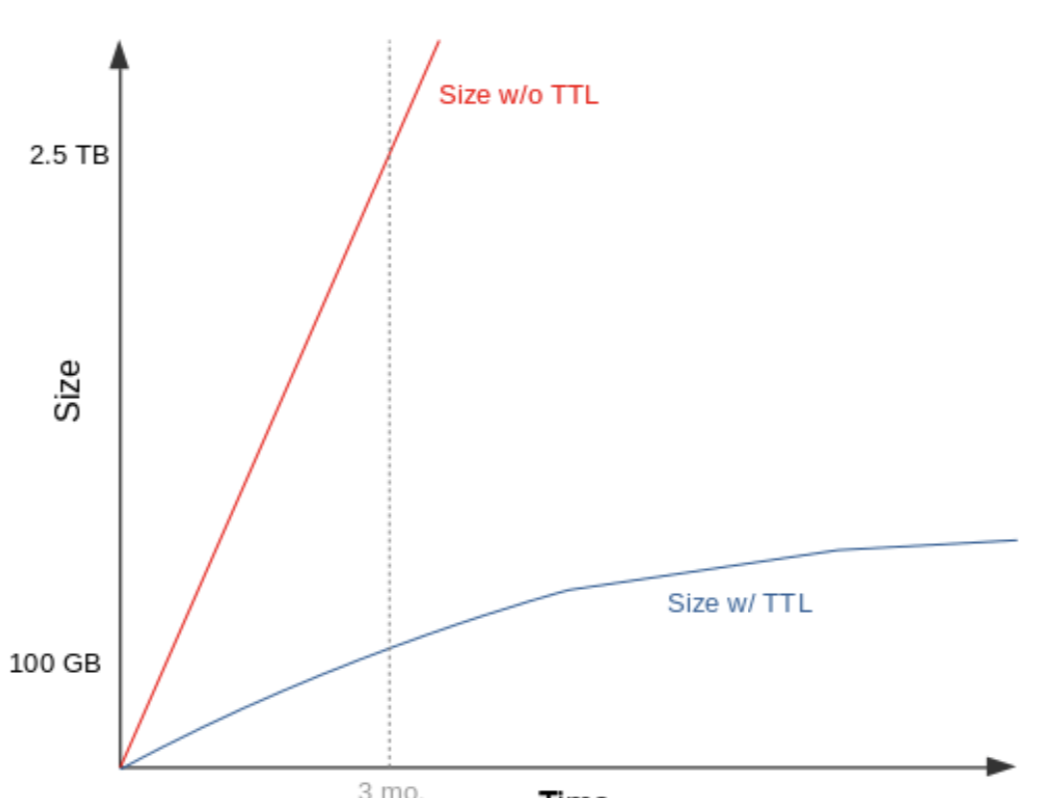
\includegraphics[width=0.4\linewidth]{images/pilot/data-management-graph.png}
	\caption{Storage requirements with and without TTL}
	\label{fig:data-management-graph}
\end{figure}

It is difficult to compute a strict upper bound on storage requirements for an OPQ network, because the amount of storage does depend on the number of power quality anomalies experienced by the grid. That said, we did notice that storage requirements were rising much more slowly at the end of the pilot when utilizing TTL as compared to not utilizing TTL.

The largest contribution to data storage is the raw power data. In a system without TTL, raw data storage rapidly grows. The bounds on raw storage can be calculated by taking into account the sampling rate and sample size for active OPQ Boxes.

Given that OPQ Boxes were configured to sample at 12 kHz at 2 bytes per sample during the deployment, we can calculate the bounds on raw storage for 16 OPQ Boxes over 3 months without TTL as 3.1 TiB.

Given a network of 16 OPQ Boxes over the pilot deployment period with TTL, the combined data storage from all levels reached an asymptotic limit of near 100 GB.  The high rate of detections made by OPQ utilize most of the space. The reason for this is that Events store associated IML data along with each detection for high-fidelity analysis. It's also possible to observe how the AML and IML levels level off asymptomatically over time. This is a result of TTL discarding not useful data.

\subsection{OPQ provides useful adaptive optimization capabilities}
\label{sec:adaptive-optimization}

The top layer of OPQ's information architecture supports adaptive optimization: the ability to analyze previously collected data and use it to change the settings associated with data collection from OPQ Boxes.

Two areas where adaptive optimizations were utilized are identifying periodic phenomena and predictions of future phenomena. Periodic phenomena are PQ related signals that occur at regular intervals. One example of periodic phenomena is a cyclic voltage sag that was observed at one of our sensors with a period of about 34 minutes during our pilot study (Figure~\ref{fig:periodic-voltage-sags}). This periodic phenomena not only provided a classification of an interesting pattern, but also helped optimize the OPQ system for capture of future phenomena. Several system wide optimizations are utilized.

\begin{figure}[H]
    \centering
    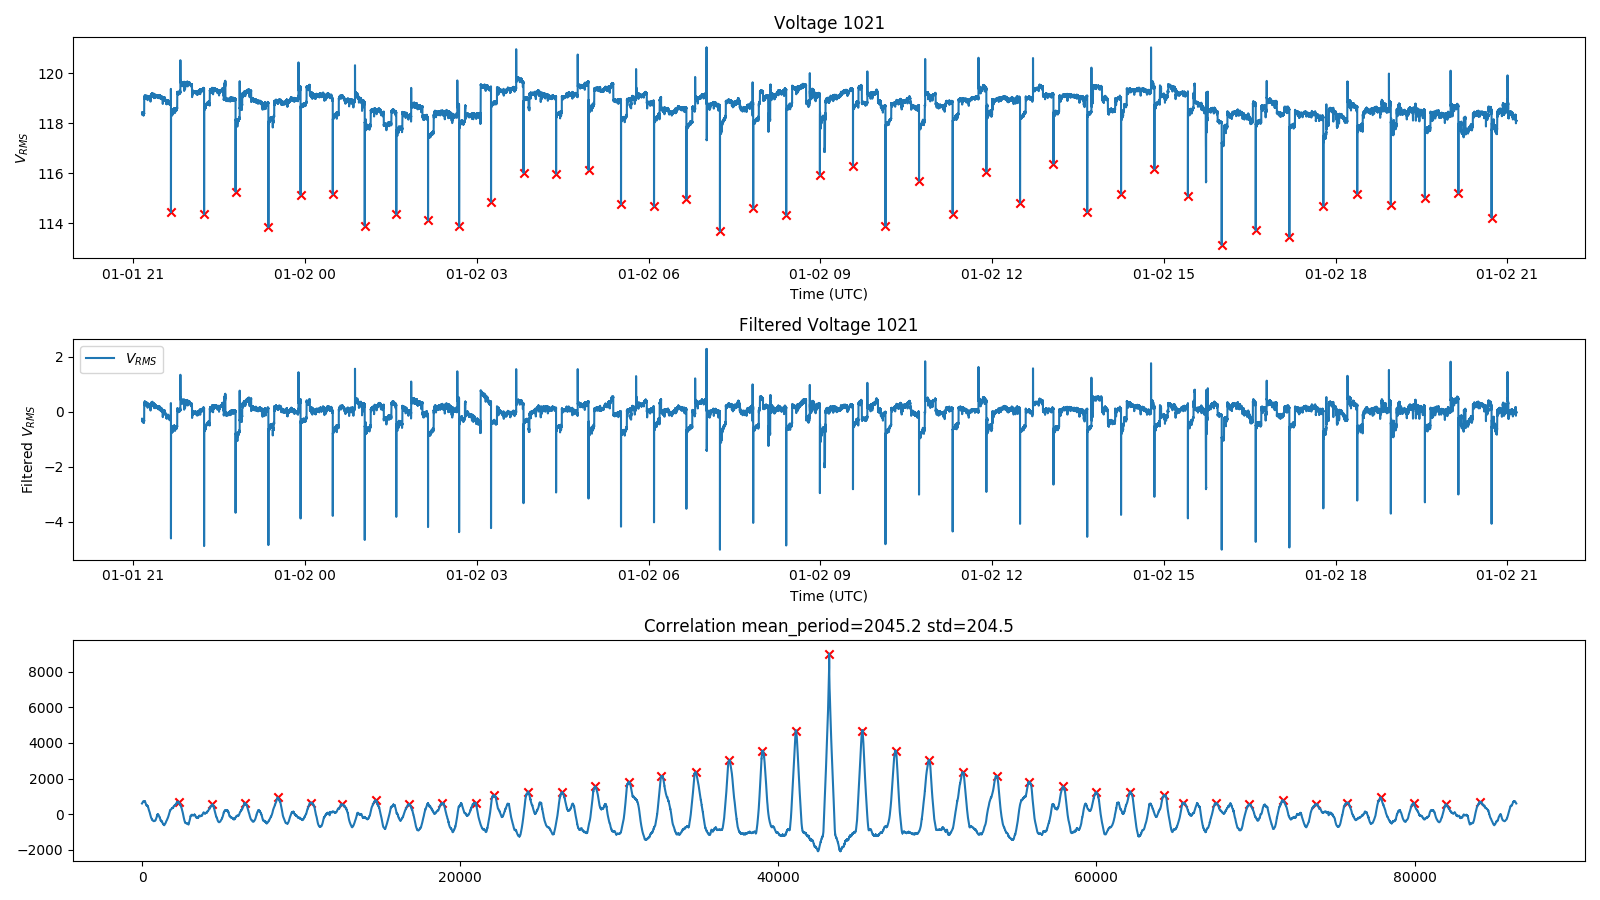
\includegraphics[width=0.90\linewidth]{images/pilot/periodic-voltage-sags.png}
    \caption{Detection of Periodic Voltage Sags}
    \label{fig:periodic-voltage-sags}
\end{figure}

First, classified periodic phenomena are used to generate future phenomena. Future phenomena are a prediction of future signals of interest. When a prediction is made, the system will automatically increase sampling fidelity for the predicted sensor during the time window of the prediction. In particular, the measurement rate is increased from 1 measurement per second to 6 measurements per second providing higher fidelity data. Detection thresholds are also decreased, making it more likely that the predicted signal will be observed even if it is of low magnitude.

Second, the increase in detection sensitivity makes it more likely that sub-threshold signals of interest will be classified. For example, the increased detection sensitivity allowed us to observe and classify a periodic voltage sag that would not have been detected by our normal classifier due to the small magnitude of the sag.

This creates a positive feedback loop whereas periodic phenomena become more accurate, future phenomena become more accurate. As future phenomena become more accurate, periodic phenomena become more accurate.







\section{Conclusions and Future Directions}
\label{sec:conclusions}

This project has produced both hardware and software for power quality monitoring with a variety of innovations.  Our OPQ Boxes collect frequency, voltage, THD, and transients with high fidelity, and at a cost that is generally 10x to 100x cheaper than current commercial offerings (though these commercial offerings offer a variety of features not available from OPQ Boxes, so the appropriate choice depends upon the needs of the user).

Our sensor network provides real-time, two-way communication between the sensor nodes (OPQ Boxes) and their cloud services, providing several innovative features for power quality monitoring. The OPQ triggering system exploits temporal locality to request high fidelity data from neighboring boxes when one exceeds a threshold, enabling our network to detect and analyze data that would have been unreported by a naive, threshold-based approach. The OPQ Information Architecture enables Actors at the Phenomena Layer to control sensitivity settings of individual OPQ Boxes in order to improve data collection when power quality anomalies have been predicted.

Our sensor network is designed to efficiently use network and storage resources. Two way communication enables OPQ Boxes to send low fidelity summary statistics on power quality at one second intervals, which can be used by cloud-based services to decide whether to request high fidelity data.  Our TTL mechanism implements a "use it or lose it" approach to cloud-based data, which in our pilot study reduced cloud storage requirements by over ten-fold.

Our pilot study has provided evidence that OPQ sensor networks can provide useful new support for understanding grid stability, particularly in grids with distributed, intermittent renewables. This in part because OPQ Boxes are suitable for installation at the residential level: installation requires only an available wall socket and WiFi connection, no electrician or GPS line-of-sight required. Finally, the low cost of OPQ Boxes means mass deployment across a neighborhood is not financially infeasible.

One future goal is to partner with an organization that can enable OPQ Boxes to be produced at volume. We made the OPQ Boxes by hand for the pilot study, and although we have had numerous requests for OPQ Boxes, we do not possess manufacturing capacity.

With manufacturing capacity will come the ability to deploy OPQ sensor networks at higher scale. We believe that a single sensor network can easily scale to hundreds of boxes before bandwidth and processing constraints become an issue. To scale to many thousands of boxes, we believe a federated approach would work in which individual OPQ sensor networks communicate their findings to each other. Those networks could be designed around natural grid boundaries such as substations.

A second goal is to explore ways to combine OPQ sensor networks with more traditional power quality monitoring tools and standards, such as PQDIF. For example, it is possible that OPQ analyses could be improved with access to additional power data such as current, phase angle, and so forth.

A third goal is to build Actors that operate not only on power quality data but also environmental data such as wind, temperature, humidity, and insolation.  These additional data streams could yield valuable mechanisms for creating Predictive Phenomena for power quality anomalies associated with renewable energy sources. Ultimately, such understanding could lead to ways to significantly increase the amount of distributed renewable energy that can be incorporated into electrical grids.

To conclude, a recent paper by Mohsenian et al \cite{mohsenian-rad_distribution_2018} states, "the main challenge is to go beyond manual methods based on the intuition and heuristics of human experts...it is crucial to develop the machine intelligence needed to automate and scale up the analytics on billions of PMU measurements and terabytes of data on a daily basis and in real time." We believe that the OPQ sensor network represents a small step along the path toward that future.





% Bibliography
\reftitle{References}
\bibliographystyle{mdpi}
\bibliography{opq}

\end{document}

